\chapter{Refinement of the INTERLACE Business Logic Specification}
\label{ch:UpdateBLS}

\vspace{-1cm}
\begin{center}
Paolo Dini, Luca Carboni, Giuseppe Littera, Egon B\"orger and Chrystopher Nehaniv
\end{center}

\section{Context and Overview}
The business logic specification provided in Deliverable D2.1 \cite{INTERLACE_D21} concerns user-initiated transactions. Although this is a subset of all possible operations (initiated by the users or by the System, which we refer to as $SysAdmin$) that a mutual credit system platform must support, it is a viable starting point for testing an initial executable CoreASIM model. D2.1 did not provide all the details of the transaction request operations, it left their specification at a fairly abstract level. This chapter provides the next step in the iterative refinement of the specification in the form of a detailed description of the Permissioning workflow, whose implementation as part of the CoreASIM model is then described in Chapter \ref{ch:CoreAsimImplementation}. The description of the Permissioning iterative refinement relies on graphical and tabular depictions of the variables and functions involved. As this reflects the process that was used to build a shared understanding within the INTERLACE team itself, it is hoped that it will also make it easier for newcomers to the INTERLACE open source community to understand the implementation and the logic behind it.

At the highest level the INTERLACE transactional platform is a dynamic information system that interacts with a database at the backend and with live users at the front-end. As already discussed in D2.1, the transaction engine relies on many categories of concepts that, together, constitute the domain model of the system. According to the ASM methodology \cite{BoergerStaerk2003,BoergerRaschke2018}, these have been subdivided into ASIMs comprised of rules, programs, and various kinds of functions. Whereas concepts such as `user' or 'transaction amount' are immediately clear, many more concepts and data structures are needed to specify and model the system. Before we get into the details, it helps to introduce three high-level perspectives through which the transaction engine can be characterized as an abstract machine and as a social construct: privacy (private-public dichotomy), dynamics (frequency domain), and transaction workflow already mentioned (time domain).

\begin{figure}[h]
\vspace{-0.5cm}
\centering
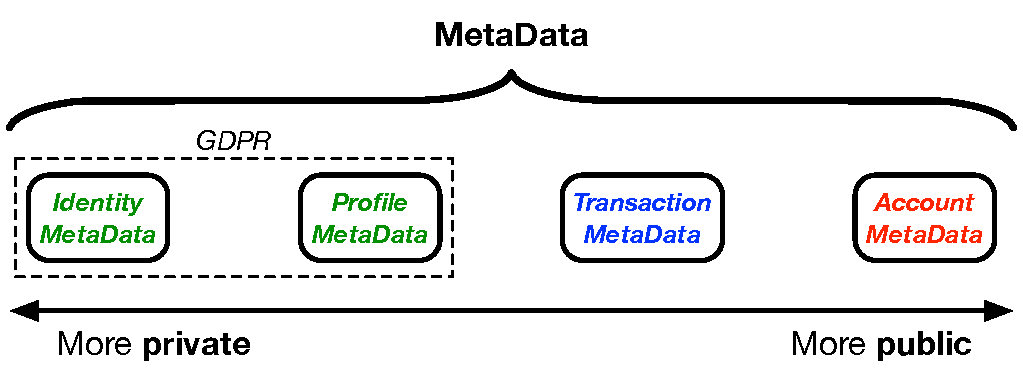
\includegraphics[width=12cm]{Figures/Private_Public_MetaData}
\caption{\small\textbf{Relative privacy of different types of meta-data of the INTERLACE transaction engine}}
\label{fig:privatepublicmetaData}
\vspace{-0.5cm}
\end{figure}

The first principle that influences the architecture of the system at a global level is the need to comply with the GDPR directive. Figure \ref{fig:privatepublicmetaData} shows how from this point of view the Transaction MetaData can be regarded as more public than the Account MetaData since it only contains a memo describing the transaction. The figure also shows that sub-dividing the meta-data in this manner makes it possible to limit the need for GDPR compliance\footnote{General Data Protection Regulation: \url{https://www.eugdpr.org/}} only to the Identity and Profile MetaData. Second, in a physics context the level of dynamicity of the variables could be described as the characteristic frequency (or its inverse, time-scale) at which different kinds of variables change as the transactional workflow is carried out. Figure \ref{fig:staticdynamicmetadata} shows how this principle applies to the system's meta-data.

\begin{figure}[h]
\vspace{-0.5cm}
\centering
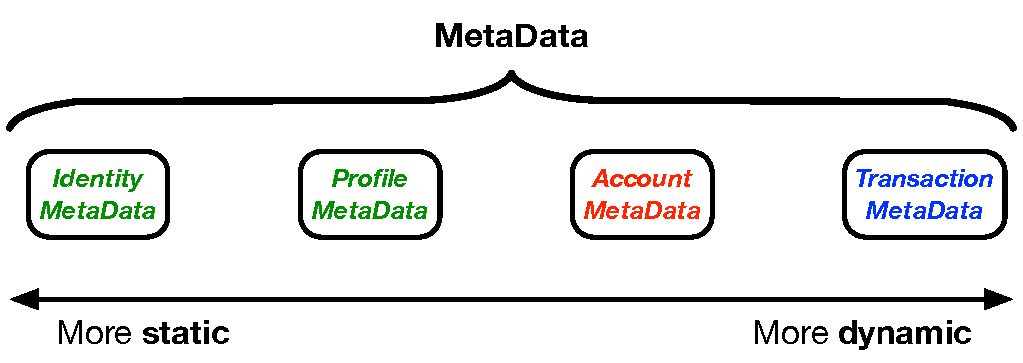
\includegraphics[width=12cm]{Figures/Static_Dynamic_MetaData}
\caption{\small\textbf{Relative dynamicity of different types of meta-data of the INTERLACE transaction engine}}
\label{fig:staticdynamicmetadata}
\vspace{-0.5cm}
\end{figure}

Third, Figure \ref{fig:transactabilitywkflow} shows the high-level view of the transaction workflow, including how the PreviewRequest and PerformRequest rules specified in D2.1 map onto it. The process starts on the left of the figure, when a user or $SysAdmin$ initiates the request for a transaction. The request must pass the three tests shown: Transfer Types, Account Connectivity and, in Inter-Circuit operations, the euroFee is calculated and shown to the user. At this point the user is shown a preview screen that summarizes all the transaction data. When the user issues the command to proceed, the first two tests are repeated and a final test on the account limits (e.g.\ sufficient funds) is performed. If also this fourth test is passed, the transaction is executed.

\begin{figure}[h]
\centering
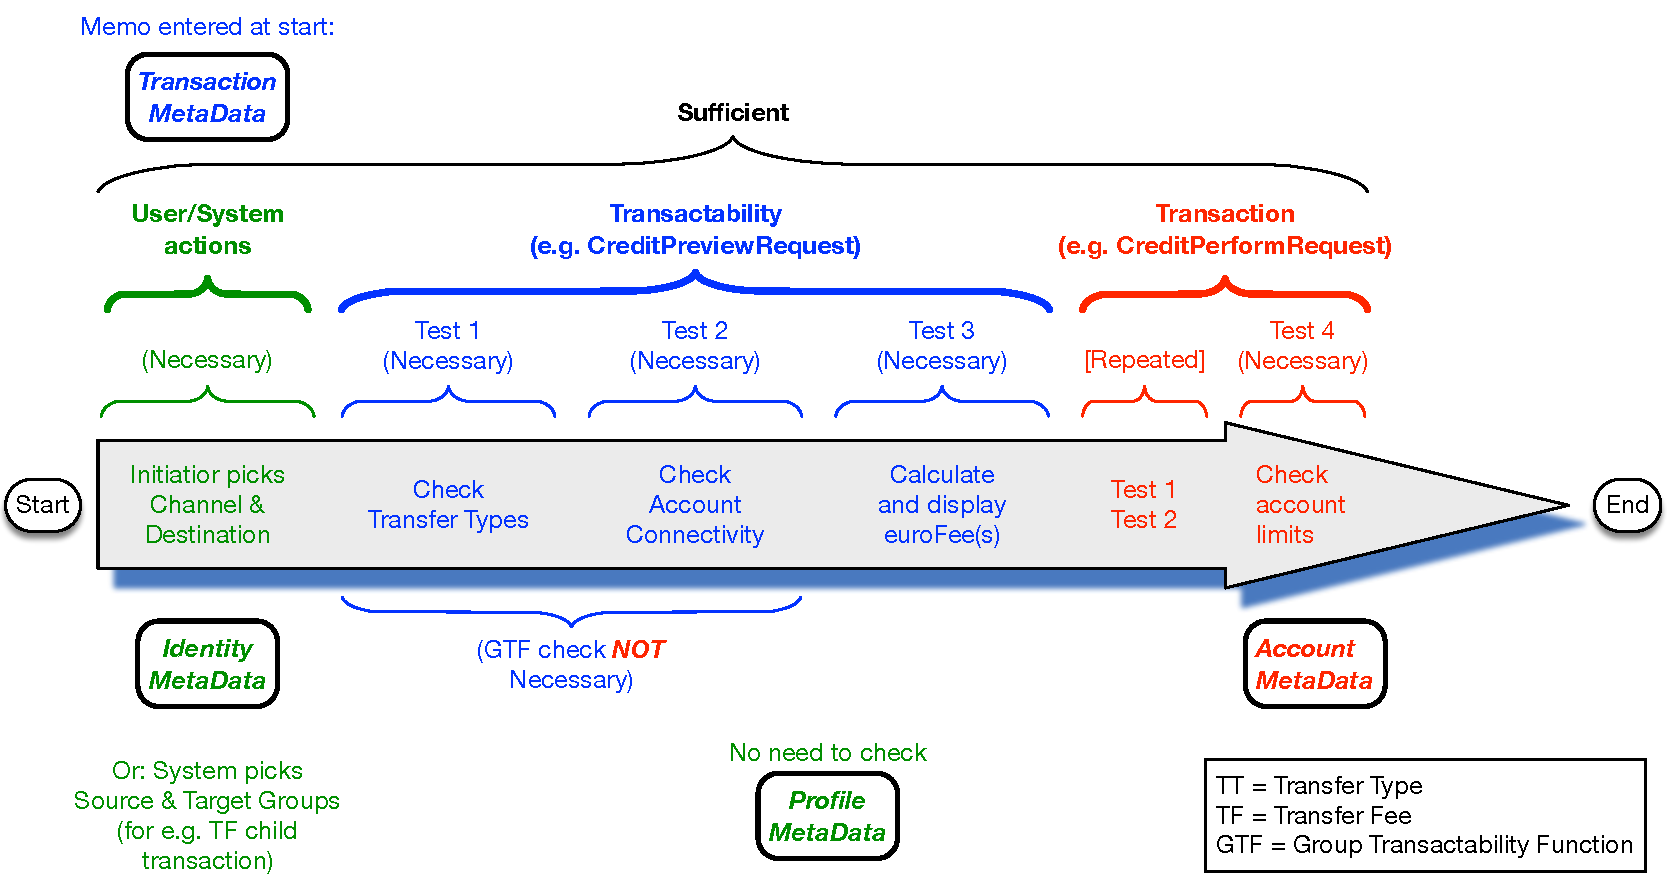
\includegraphics[width=17.5cm]{Figures/Transactability_Workflow}
\caption{\small\textbf{High-level workflow of the Permissioning process for user- or system-initiated transactions}}
\label{fig:transactabilitywkflow}
\end{figure}

In the following, first we provide a taxonomy of all the terms and concepts used and needed by the model, and then proceed to explain each step of the transaction workflow.


\section{Permissioning Model Taxonomy}
\subsection{Users and Groups}
Users are organized by user types called `Groups'. Consistently with the Appendix, in mathematical notation a $Group$ is a set of $group$s, such that $group \in Group$. However, also an individual $group$ is a set, specifically it is a set of users of the same type. Therefore, the group $Retail$ is capitalized, whereas a single shop is a $retail$. In the original Sardex platform not much distinction is made between users and groups. However, in the current INTERLACE specification we do need to discriminate between them.

\begin{quote}
\vspace{-0.3cm}
\small
For example, when describing a Debit transaction use case, at the User level the Seller initiates the Debit transaction to draw funds from the Buyer's account. In this scenario, therefore, the Seller is the $fromUser$ and the Buyer is the $toUser$. However, at the Group level things are different. As part of the transactability tests to be described fully in later sections, to each group that initiates a transaction ($fromGroup$) is associated a set of groups that can be on the receiving end of that transaction. In the case of a Debit transaction, whereas the \emph{request} goes to the Buyer, the receiving end of the transaction is not the Buyer, it is the Seller. Therefore, in a Debit operation $fromGroup$ = Seller, and $toGroup$ = Seller too!
\vspace{-0.3cm}
\end{quote}

The possible confusion created by debit transactions is resolved at the level of the accounts. See Section \ref{sec:intlevels}. The original Sardex system divided its users into 29 different groups. This generated a great deal of complexity that is drastically reduced in the INTERLACE version of the platform. The new user type taxonomy involves only 9 groups, as shown in Table \ref{tab:groups}.

%\setcounter{table}{0}
\setlength{\tabcolsep}{10pt}
\begin{table}[h]
\vspace{-0.3cm}
\begin{centering}
\small
{
\begin{tabular}{ r | l  }
\hline
\textbf{Group}	& \textbf{Description of Element of Group} \\
\Xhline{1.5pt}
$Welcome$ & User who has joined and signed the contract, but has not yet been cleared to start trading \\
\hline
$Retail$ & Retailer who can \emph{only} participate in B2C operations (not B2E and not B2B) \\
\hline
$Company$ & Company, which could be a retailer, that can use B2E and B2B but \emph{not} B2C \\
\hline
$Full$ & This group has all the functions of $Retail$ and of $Company$ \\
\hline
$Employee$ & Employee of a $company\in Company$ or of a $full \in Full$ \\
\hline
$On$\_$Hold$ & User whose privileges have been suspended (for whatever reason) \\
\hline
$Consumer$ & Person not registered to the circuit who can only interact through B2C Use Case 2 \\
\hline
$Consumer$\_$Verified$ & $consumer$ who has registered and can now also purchase with SRD (B2C Use Case 3)  \\
\hline
$MNGR$ & Manager of the circuit (e.g.\ Sardex S.p.A.) acting as a $company$ rather than $SysAdmin$ \\
\Xhline{1.5pt}
\end{tabular}
}
\caption{\small\textbf{New user types (groups) for the INTERLACE platform}}
\label{tab:groups}
\end{centering}
\vspace{-0.7cm}
\end{table}

$SysAdmin$ is not defined explicitly as a group, in this model, although technically it too is a user type. $SysAdmin$ has special privileges, some of which are discussed where relevant in what follows. We do not use lower-case for $MNGR$ and $SysAdmin$ because there is only one of each.

\subsection{Currencies and Channels}
As shown in Figure \ref{fig:currchan}, the Sardex/INTERLACE platform supports transactions in both Sardex credits (SRD) and Euros (EUR) over two kinds of channels. `Service' refers to transactions mediated either by a computer (web application) or a mobile phone (either a web application or a phone App). `POS' means `Point of Sale' and refers to the standard terminal used by retailers that accepts credit or debit cards, through which SRD transactions can be routed via an API. The figure also shows the four possible $\{ currency, channel \}$ combinations that we need to support in the definition and implementation of the permissioning tests discussed in the next sections.

\begin{figure}[h]
\vspace{-0.3cm}
\centering
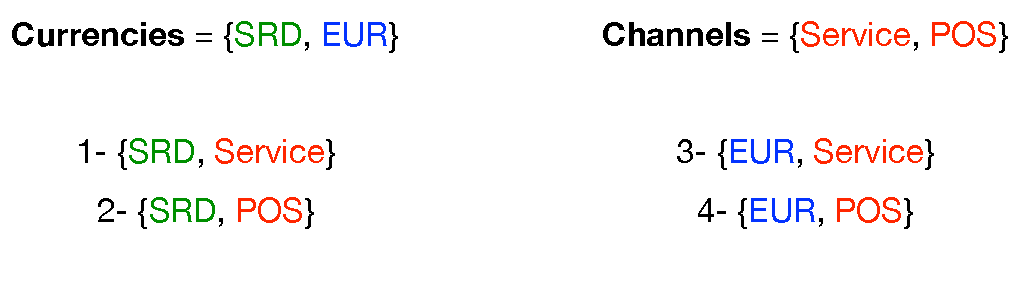
\includegraphics[width=10cm]{Figures/Curr_Chan}
\caption{\small\textbf{Currencies and channels supported by the platform}}
\label{fig:currchan}
\vspace{-0.5cm}
\end{figure}

\subsection{Accounts}
As shown in Table \ref{tab:accounts}, the accounts implemented in the model reflect the current operations of the Sardex system and the needs of a wide range of business operations and interactions. Some of the account types, for example MIRROR, may be phased out as the high-level architecture of the family of Sardex circuits grows and different algorithms replace the current strict controls on the balance of payments between different circuits. Also an account can be referred to as $fromAcct$ or $toAcct$ depending on its role in the transaction. See Section \ref{sec:intlevels}.

\setlength{\tabcolsep}{10pt}
\begin{table}[htbp]
\vspace{-0.3cm}
\begin{centering}
\small
{
\begin{tabular}{ r | l  }
\hline
\textbf{Account}	& \textbf{Description} \\
\Xhline{1.5pt}
$CC$ & Standard Sardex credits (SRD) account \\
\hline
$DOMU$ & SRD account used for larger operations, such as for real estate or capital equipment\\
\hline
$MIRROR$ & Account controlled by $MNGR$, used for inter-circuit purchases \\
\hline
$Income$ & Statistical EUR account owned by $retail$ or $full$ that collects B2C payments\\
\hline
$Prepaid$ & Statistical EUR account from which the 2\% child B2C transaction fee is drawn \\
\hline
$Bisoo$ & Statistical EUR account used by $consumer$ to pay into Income \\
\hline
$Topup$ & Statistical EUR account used by $MNGR$ to recharge $retail$'s Prepaid account upon receipt of \\
&\hspace{0.5cm} EUR payment. It is recharged back to zero gradually with each B2C transaction. \\
\Xhline{1.5pt}
\end{tabular}
}
\caption{\small\textbf{New user types (groups) for the INTERLACE platform}}
\label{tab:accounts}
\end{centering}
\vspace{-0.3cm}
\end{table}

\subsection{Account Limits}
Table \ref{tab:accountLimits} shows the account limit parameters that apply to the SRD accounts CC, DOMU, and MIRROR. The credit limit is straightforward, it is the maximum negative value the account balance can reach. However, note that it is expressed as a \emph{positive} number. This is important to keep in mind for the calculations that are based on the value of this parameter. The credit limit is set at the time a user signs the contract with Sardex and is reviewed at least every year after that. The upper limit is, similarly, the maximum value the balance of the account is allowed to reach. Whereas the credit limit can be considered to be a safety measure for the circuit, the upper limit is more a safety measure for the user, since if the balance becomes too large-positive it may be difficult for the user to find ways to spend the credits in a useful time (for the user). Capacity is the maximum total sale volume that the user commits to accepting in one year. The alerts are safety buffers set by the user to alert him/her when the account balance and/or the sale volume approach these limits.

\setlength{\tabcolsep}{10pt}
\begin{table}[htbp]
\vspace{-0.3cm}
\begin{centering}
\small
{
\begin{tabular}{ r | l  }
\hline
\textbf{Account Limit Parameter} & \textbf{Description} \\
\Xhline{1.5pt}
$creditLimit$& Maximum negative SRD balance allowed (\emph{positive} number) \\
\hline
$upperLimit$ & Maximum positive SRD balance allowed (positive number)\\
\hline
$capacity$ & Maximum {\bf sale} volume allowed in one year \\
\hline
$lowBalanceAlert$ & Buffer set by user: alert if $(creditLimit + balance) < lowBalanceAlert$\\
\hline
$highBalanceAlert$ & Buffer set by user: alert if $(upperLimit - balance) < highBalanceAlert$ \\
\hline
$highVolumeAlert$ & Buffer set by user: alert if $(capacity - saleVolume) < highVolumeAlert$ \\
\Xhline{1.5pt}
\end{tabular}
}
\caption{\small\textbf{Account limit parameters}}
\label{tab:accountLimits}
\vspace{-0.3cm}
\end{centering}
\end{table}

Figure \ref{fig:accountLimitsCC} shows a visualization of the account limits that apply to SRD accounts such as $CC$. The thick vertical green arrows highlight that the calculation of the sale volume is defined as \emph{the sum of all the sales performed in one year}. In this example, the sum of all the vertical green arrows is 50,000. Figure \ref{fig:accountLimitsPrepaid} is a visualization of the $Prepaid$ EUR account, which is recharged or topped up once in a while (\euro 400 in the figure) and slowly drawn down by B2C transaction fees (see B2C Use Case 2 in Figure \ref{fig:B2C1} below).

\subsection{Operations}
As already specified in D2.1, transactions are effected through two operations: $credit$ and $debit$:
\begin{align}
Operation = \{ credit, debit \}.
\end{align}

\begin{figure}[h]
\vspace{-0.5cm}
\centering
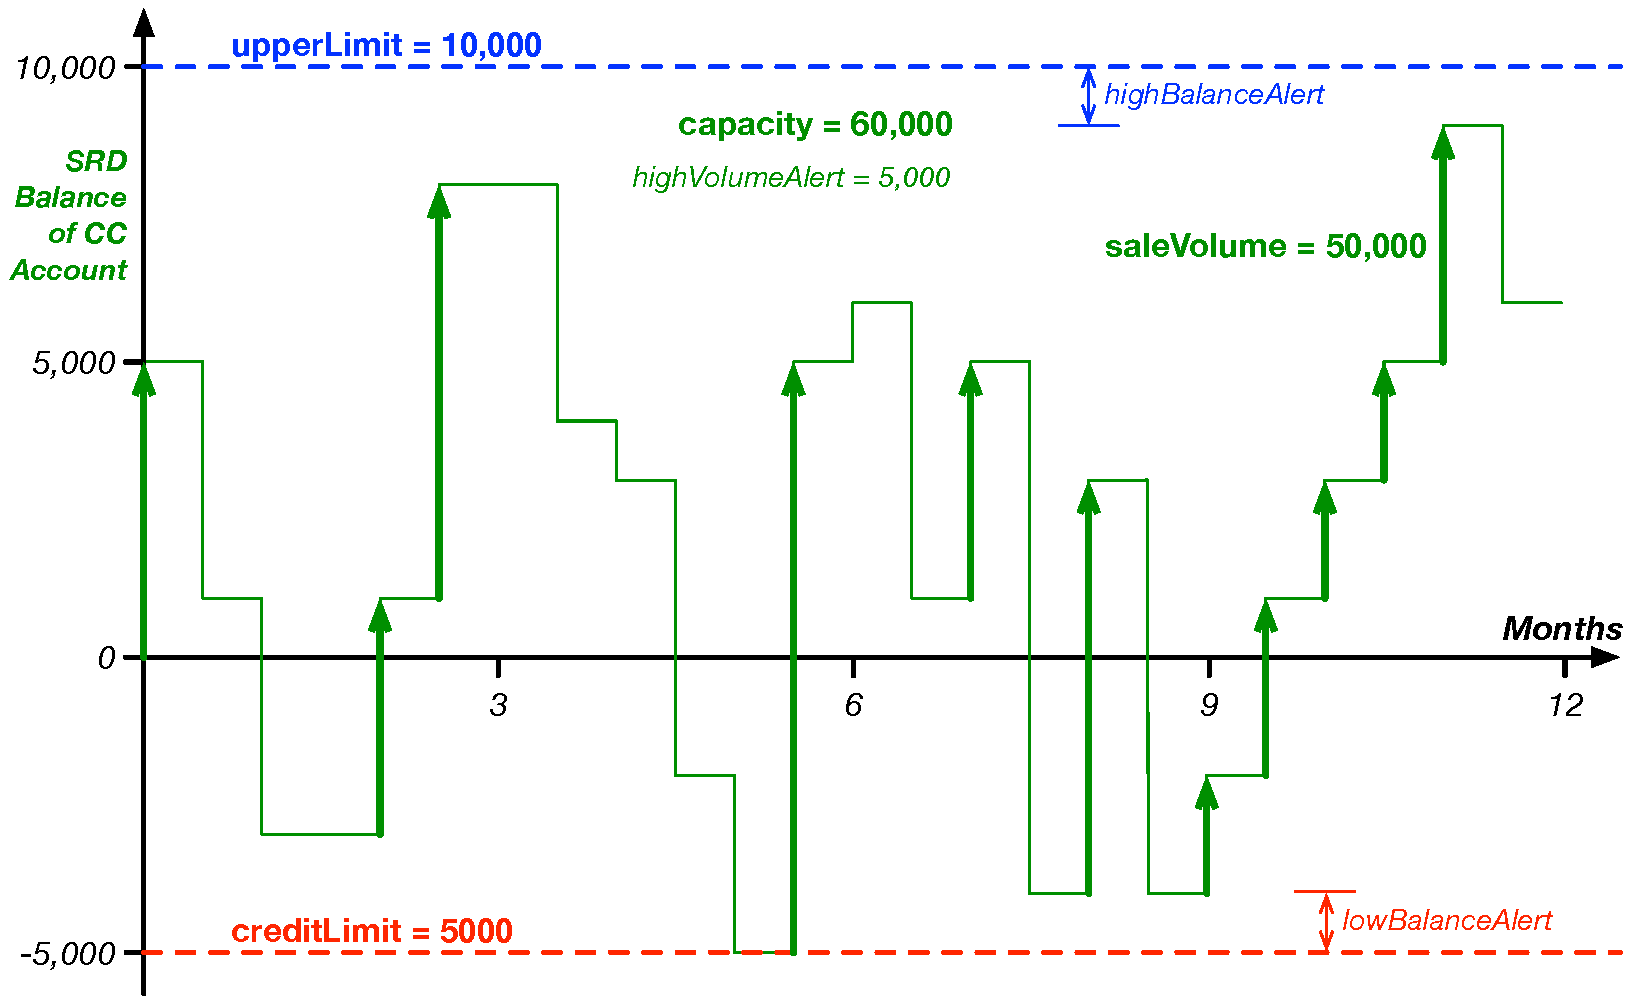
\includegraphics[width=15cm]{Figures/Account_Limits_CC}
\caption{\small\textbf{Visualization of the $CC$ account limits}}
\label{fig:accountLimitsCC}
\vspace{-0.8cm}
\end{figure}


\begin{figure}[htbp]
\vspace{-0.8cm}
\centering
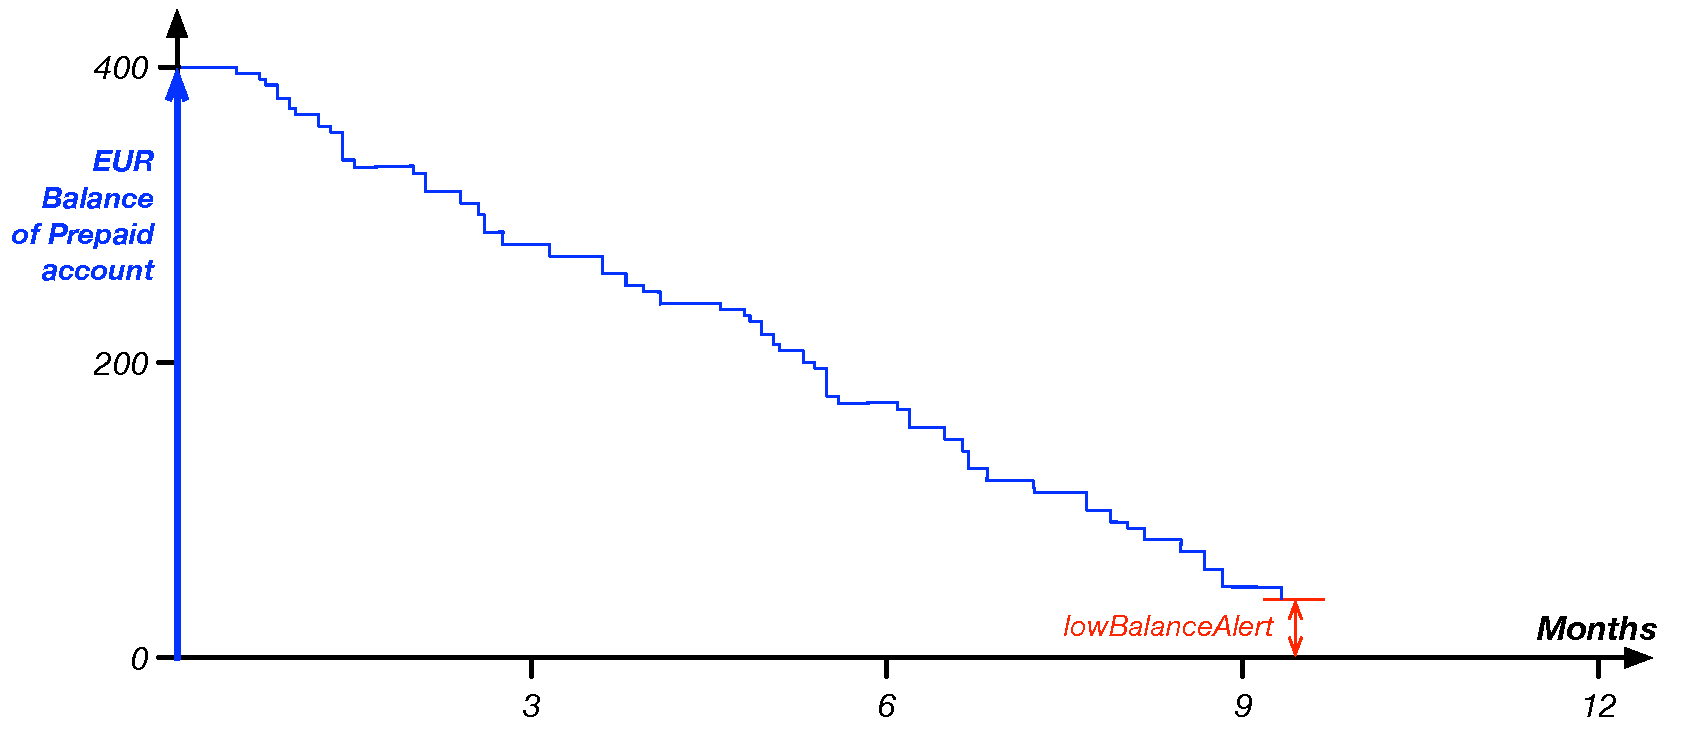
\includegraphics[width=15.6cm]{Figures/Account_Limits_Prepaid}
\caption{\small\textbf{Visualization of the $Prepaid$ account limit}}
\label{fig:accountLimitsPrepaid}
\vspace{-0.5cm}
\end{figure}


\subsection{Interaction Levels}
\label{sec:intlevels}
The interactions between circuit participants can be described from different points of view that correlate loosely to a stack view of the system. As shown in Figure \ref{fig:stack}, it is helpful to identify qualitatively the different levels of such a stack, acknowledging that it is \emph{more} than a networking communication stack in terms of scope but \emph{less} than one in terms of precision. `A' and `B' refer to the Buyer and the Seller respectively. Figure \ref{fig:stack} extends the two communication levels described in D2.1, but does so qualitatively. For the purposes of the implementation, we need a smaller set of levels but a more precise and specific vocabulary to identify the end-points of the transaction.

\begin{figure}[H]
\centering
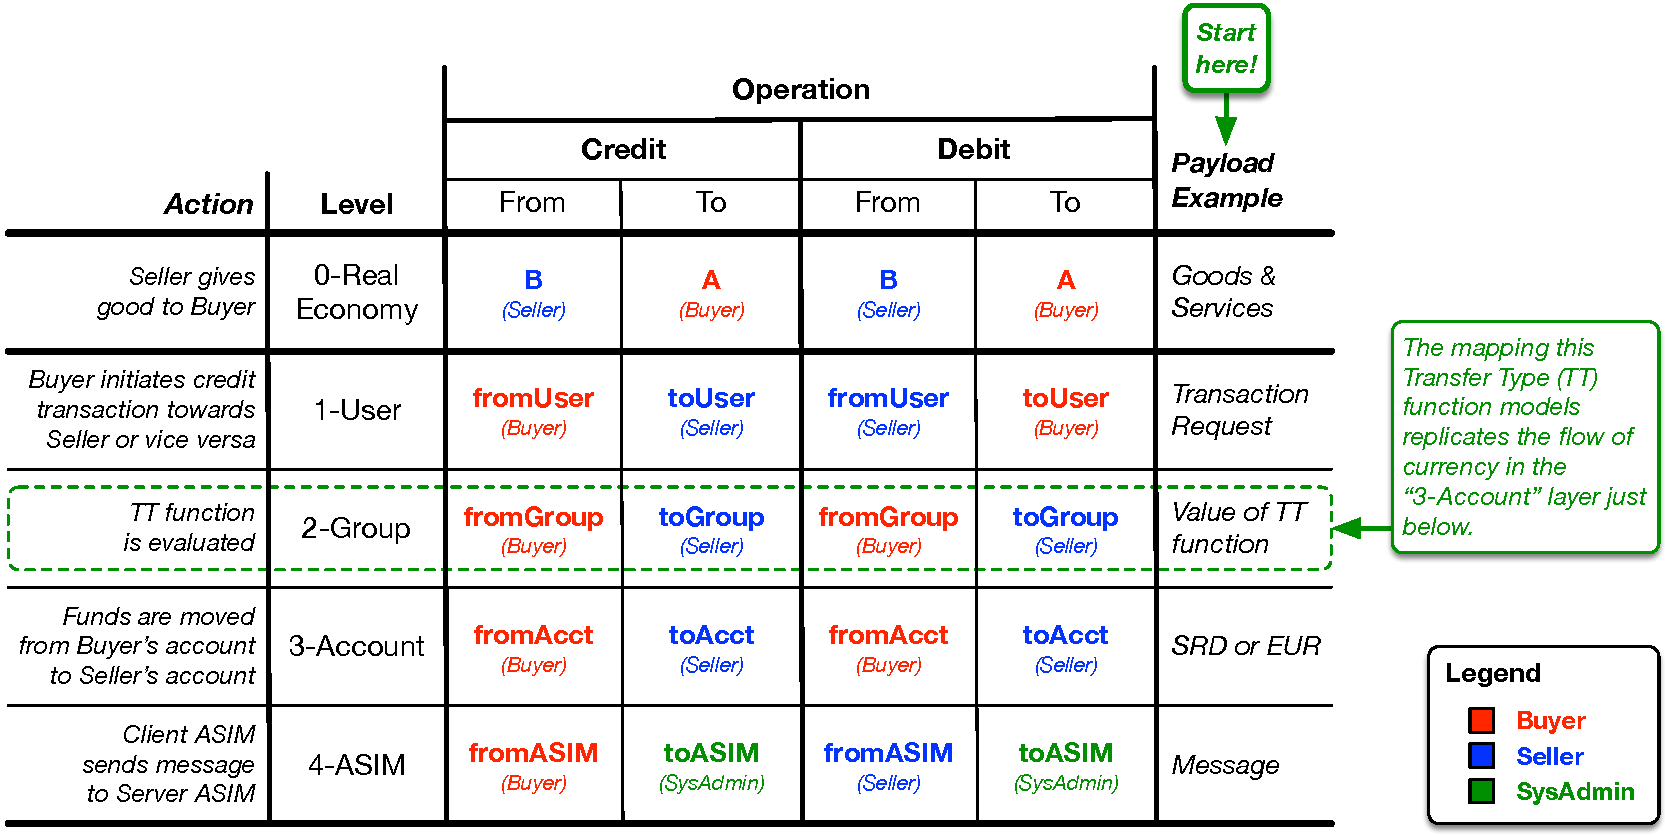
\includegraphics[width=17.5cm]{Figures/Stack}
\caption{\small\textbf{Stack view of the INTERLACE communication, economic, and financial  interactions}\\
(Stack view of from where to where the different payloads are moved in interactions)}
\label{fig:stack}
\vspace{-0.5cm}
\end{figure}

Figure \ref{fig:vocabulary} shows this additional information as concerns levels 1-4, which are labelled in the first column in the same way as in Figure \ref{fig:stack}, along with some more information. In particular, this figure could be seen to integrate aspects of Figures \ref{fig:stack} and \ref{fig:transactabilitywkflow}, with the purpose of facilitating the conceptual understanding of the specification. The different types of `MetaData' relevant to transactions are shown in the approximate position where they are polled. For example, the $\%$ of SRD accepted by a given user over 1000-EUR transaction values is part of the Profile MetaData of the $Company$ group but not the $Consumer$\_$Verified$ group's.

\begin{figure}[htbp]
\centering
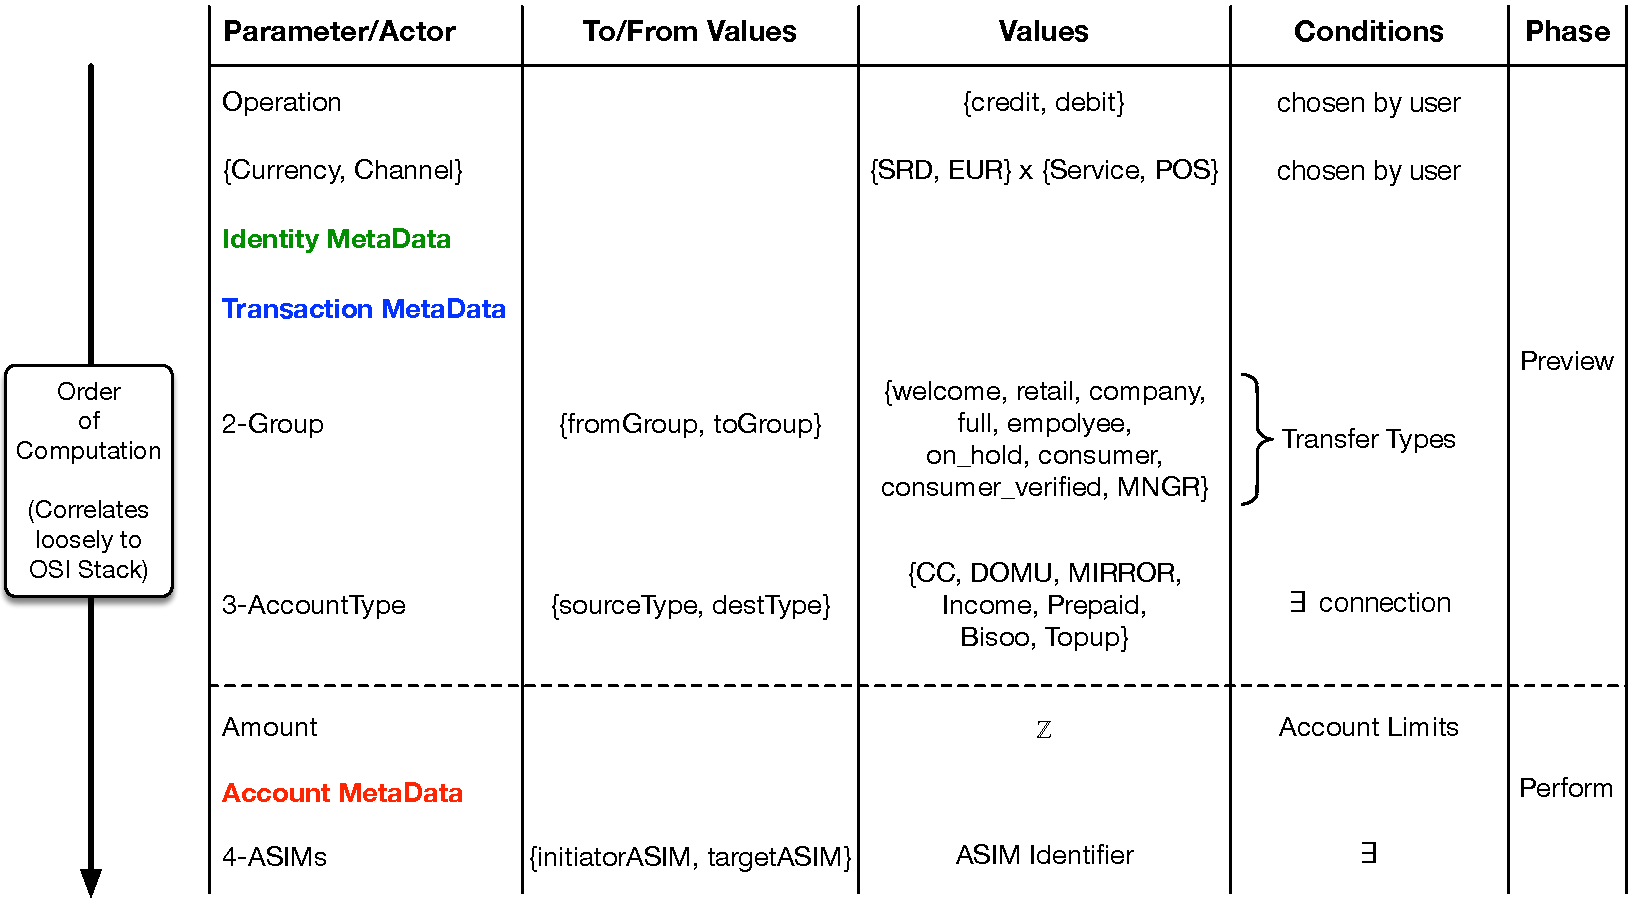
\includegraphics[width=17cm]{Figures/Vocabulary}
\caption{\small\textbf{Actors, parameters, levels, data structures, computational process, and conditions}}
\label{fig:vocabulary}
\end{figure}

\subsection{Visibility}
Figure \ref{fig:visibility} shows which groups ($toGroup$) are visible to which groups ($fromGroup$) by a `1' at the intersection of the $(row, column)$ corresponding to a choice of $(fromGroup, toGroup)$. For example, $Company$ is visible to $Employee$, meaning that $Employee$ can do a search for $Company$, but not vice versa. In this case $Employee$ is not visible due to privacy legislation.

\begin{figure}[H]
\centering
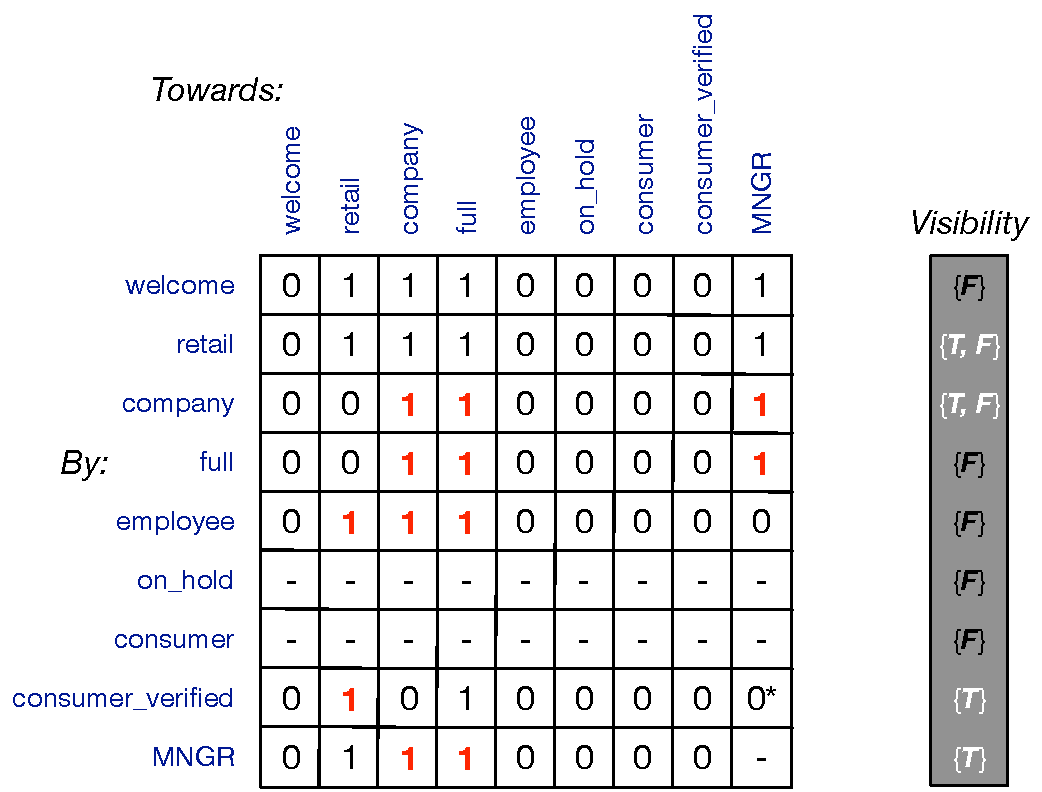
\includegraphics[width=12cm]{Figures/Visibility}
\caption{\small\textbf{Mutual visibility of different groups}}
\label{fig:visibility}
\vspace{-0.5cm}
\end{figure}

In general, transactability correlates to visibility. However, there is not a strict 1-1 relationship between them. For the example of a $company$ paying its own $employee$s as part of the B2E programme, $employee$ remains invisible to a search, but $company$ has the $username$ of the $employee$ and can perform a credit transaction to pay (part of) their salary.

On the right of Figure \ref{fig:visibility} we show that some groups are always invisible $\{ F \}$ others are always visibile $\{ T \}$, and others could be either $\{T, F\}$. For example, a company could be put in the shadow state if it has reached its maximum positive credit limit.

\subsection{B2C Operations}
This report extends the use cases covered by D2.1 by adding also the Business to Consumer (B2C) use cases. B2C was developed to increase the number and volume of transactions, i.e.\ the size of the Sardex economy, by extending the ability to transact in SRD to people not otherwise connected to the circuit. The principle involves offering the opportunity to $retail$ers to reward their EUR customers with an SRD rebate.

The amount of the reward is a percent, in SRD, of the amount in EUR paid by a $consumer$ to a $retail$, where the percent is set by $retail$ and it is an example of the $MetaData$ for this group. The reward is stored on a smart card that is offered to $consumer$ at the time of purchase. This is shown as a child transaction in B2C Use Case 2, Figure \ref{fig:B2C1}.

\begin{figure}[htbp]
\centering
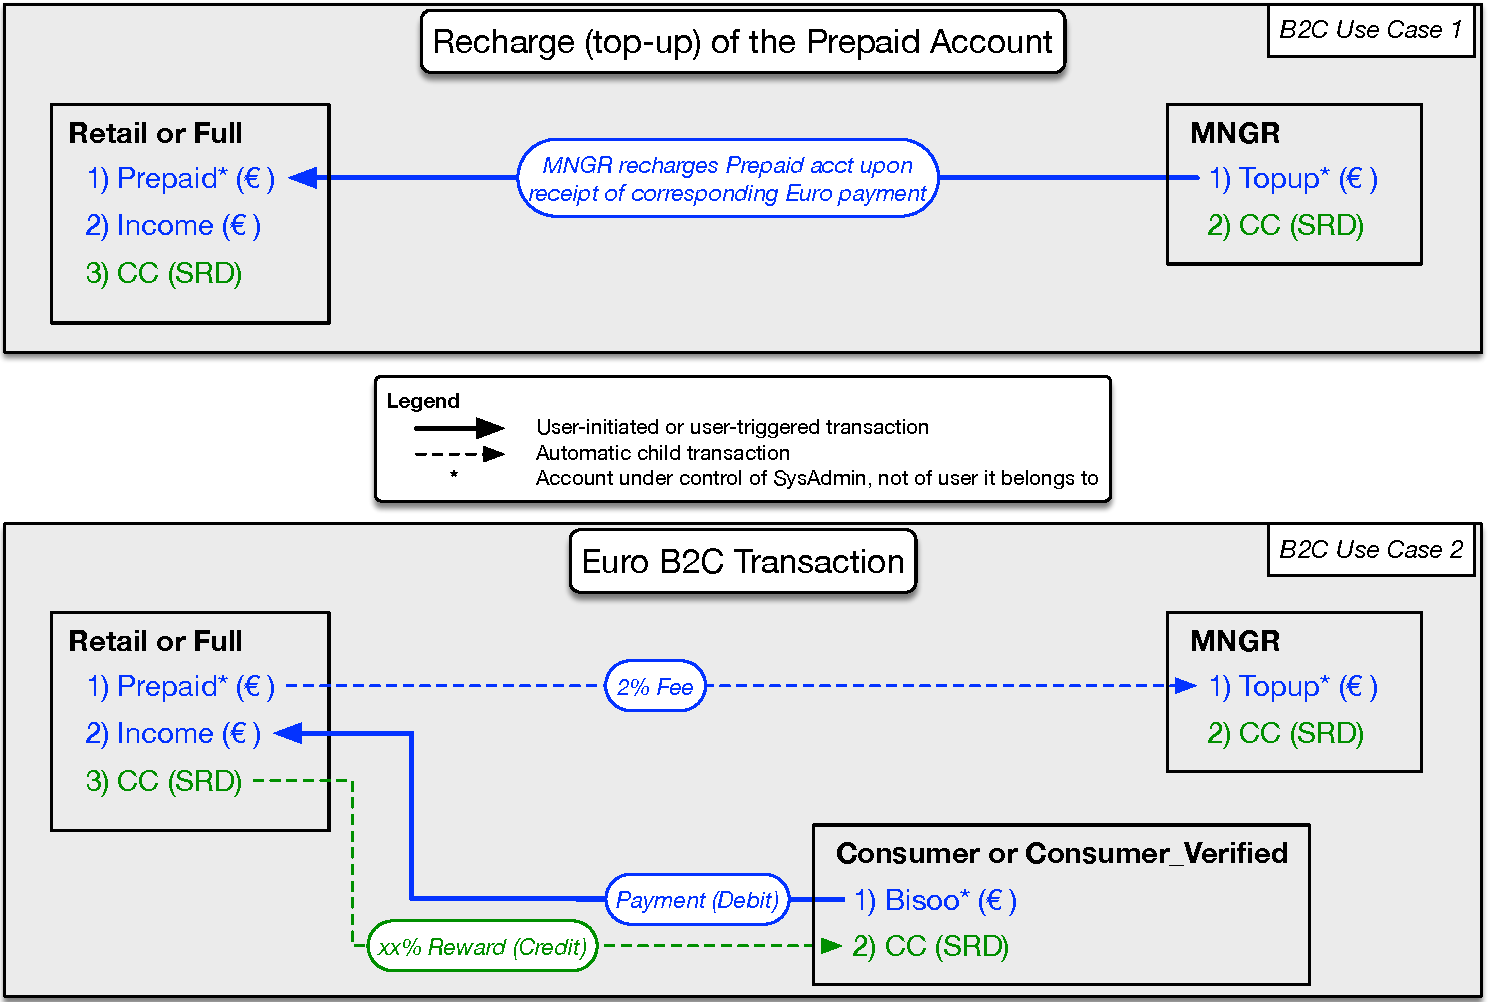
\includegraphics[width=15cm]{Figures/B2C1}
\caption{\small\textbf{Recharging of $retail$'s Prepaid account and standard B2C EUR transaction}}
\label{fig:B2C1}
\end{figure}

Use Case 2 also involves a second child transaction, a 2\% fee, in EUR, paid from $retail$'s Prepaid account to $MNGR$'s Topup account. The asterisks next to these account names, in the figure, indicate that these two accounts are \emph{owned} by these two users but are not \emph{controlled} by them. They are controlled by $SysAdmin$. These EUR accounts are `statistical' rather than `real', meaning that they simply keep track of actual EUR amounts but do not themselves hold Euros. Sardex S.p.A. would need to be a bank for that to be possible. For Use Case 2 to be executable, for a given $retail$er, its Prepaid account needs to have sufficient funds. When it runs out of statistical Euros, $retail$ can pay $MNGR$ some amount of Euros using any of the standard payment systems, through a bank or a payment service provider like PayPal. This triggers Use Case 1, also shown in Figure \ref{fig:B2C1}.

\begin{figure}[h]
\centering
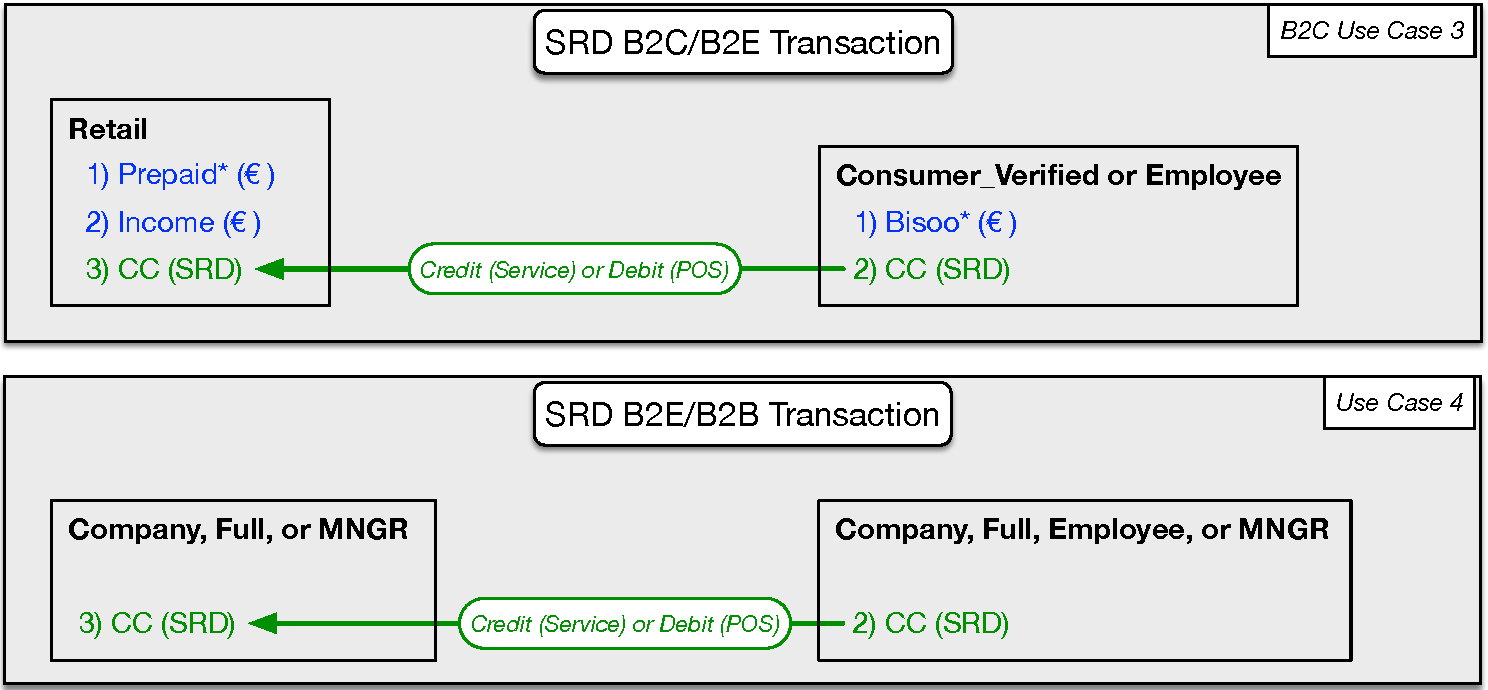
\includegraphics[width=15cm]{Figures/B2C2}
\caption{\small\textbf{SRD transactions for B2C, B2E, and B2B users}}
\label{fig:B2C2}
\end{figure}

Figure \ref{fig:B2C2} shows the SRD transaction a $consumer$ can perform, i.e.\ the spending of the SRD accumulated as rewards, once they have registered and have become $consumer$\_$verified$. The figure also shows that Use Case 3 is relevant also to $employee$s (B2E) and that Use Case 4 is relevant to both B2E users and to non-$retail$ company users (B2B).

\subsection{Initial Account State}
Table \ref{tab:InitialAccountSets} shows the initial allocation of accounts to the different user groups. The allocation is `initial' because  depending on the history of a given user the number of its accounts could change. For legal reasons, as a general principle \emph{change} can only mean \emph{increase}. In other words, once a user has become the owner of an account it can never be taken away from them, even if, for example, its access to it is suspended due to misbehaviour. Another example is a $Retail$ user who upgrades to the $Full$ group and a year later changes its mind and goes back to $Retail$. It will retain its DOMU account even if it won't be able to use it anymore.

{\bf Note: Each user can have no more than one account of a given type.}

\begin{table}[h]
\vspace{-0.5cm}
\begin{centering}
\small
{
\begin{tabular}{ r | l  }
\hline
\textbf{Group}	& {\bf Initial Account Set} \\
\Xhline{1.5pt}
$Welcome$	& $\{ \}$ \\
\hline
$Retail$		& $\{ CC, Prepaid^*, Income \}$ \\
\hline
$Company$	& $\{ CC, DOMU, Prepaid^* \}$ \\
\hline
$Full$		& $\{ CC, DOMU, Prepaid^*, Income \}$ \\
\hline
$Employee$	& $\{ CC \}$ \\
\hline
$On$\_$Hold$	& $\{ CC, DOMU, Prepaid^*, Income \}$ \\
\hline
$Consumer$	& $\{ CC, Bisoo^* \}$ \\
\hline
$Consumer$\_$Verified$ & $\{ CC, Bisoo^* \}$ \\
\hline
$MNGR$ 		& $\{ CC, Topup^*, MIRROR \}$ \\
\Xhline{1.5pt}
\end{tabular}
}
\caption{\small\textbf{Initial sets of accounts assigned to the groups}\\ (*Indicates an account under the control of $SysAdmin$, not of the user it belongs to.)}
\label{tab:InitialAccountSets}
\end{centering}
\vspace{-1cm}
\end{table}

The Prepaid account shown for $Company$ does not relate to B2C operations but to inter-circuit trade, which also involves a euroFee.

\section{Transactability Workflow}
\subsection{Identity MetaData}
Table \ref{tab:IdentityMetaData} collects the identity meta-data for all the groups. $MemberID$ is a unique identifier. $email$ and $phone$ are arrays to support multiple values of each. These values are set at registration and cannot be changed by the user.

The meta-data variables are not capitalized because they are assumed to be singletons: for a given member, e.g.\ a $company$, there is only one $memberID$. However, since there are many $memberID$s, one for each member, we could also say that $memberID \in MemberID$. Since there are cases where a user may have more than one meta-data variable, for example a company with more than one phone number, this is indicated in the Type column as an array, i.e.\ `String[ ]'.

\begin{table}[H]
\vspace{-0.5cm}
\begin{centering}
\small
{
\begin{tabular}{ r | c | l | l }
\hline
\textbf{Group}	& {\bf Identity MetaData} & {\bf Type} & {\bf Description} \\
\Xhline{1.5pt}
$Welcome$, $Retail$, $Company$,	& {\bf memberID}			&Integer	& Unique member identifier \\
$Full$, $Employee$, $On$\_$Hold$,	& {\bf email}				&String[]	& e-mail address \\		
$Consumer$\_$Verified$, $MNGR$	& {\bf phone}				&String[]	& phone number(s) \\
\hline
$Consumer$	& {\bf memberID}	&Integer & Unique member identifier \\
\Xhline{1.5pt}
\end{tabular}
}
\caption{\small\textbf{Identity MetaData for all the groups}}
\label{tab:IdentityMetaData}
\end{centering}
\vspace{-1cm}
\end{table}

\subsection{Profile MetaData}
Tables \ref{tab:ProfileMetaData1} and \ref{tab:ProfileMetaData2} show the profile meta-data, some of which the user can inspect and edit. For example, the user may wish to include his/her personal name in addition to the company name.

\setlength{\tabcolsep}{10pt}
\begin{table}[H]
\begin{centering}
\small
{
\begin{tabular}{ r | c | l | l }
\hline
\textbf{Group}	& {\bf Profile MetaData} & {\bf Type} & {\bf Description} \\
\Xhline{1.5pt}
			& \emph{(Obligatory MetaData)} & & \\
\cline{2-2}
$Welcome$	& {\bf entityName}$^*$		&String	& Legal entity name \\
			& {\bf entityAddress}$^*$		&String	& Legal entity's street address \\
			& {\bf gps}$^*$				&Double[]	& Legal entity's GPS coordinates \\			
			& {\bf VAT}$^*$				&String	& Legal entity's VAT number \\
			& {\bf capacity}				&Double	& Commitment to maximum yearly SRD volume \\
			& {\bf capacityDate}			&DateTime & Date capacity was set \\
\cline{2-2}
			 & \emph{(Optional MetaData)}& & \\
\cline{2-2}
			& {\bf firstName}$^*$			&String	& First name \\
			& {\bf surName}$^*$			&String	& Surname \\
\Xhline{1.5pt}
			& \emph{(Obligatory MetaData)} & & \\
\cline{2-2}
$Retail$		& {\bf entityName}$^*$		&String	& Legal entity name \\
			& {\bf entityAddress}$^*$		&String	& Legal entity's street address \\
			& {\bf gps}$^*$				&Double[]	& Legal entity's GPS coordinates \\			
			& {\bf capacity}				&Double	& Commitment to maximum yearly SRD volume \\
			& {\bf capacityDate}			&DateTime & Date capacity was set \\
			& {\bf rewardRate}$^{**}$		&Double	& \% reward rate to consumer, in SRD \\
			& {\bf euroFee}				&Double[]	& \% fee on B2C EUR sales, in EUR \\
			& {\bf acceptanceRate}$^{**}$	&Double	& Rate of SRD acceptance in consumer purchases\\
\cline{2-2}
			 & \emph{(Optional MetaData)}& & \\
\cline{2-2}
			& {\bf firstName	}$^*$			&String	& First name \\
			& {\bf surName}$^*$			&String	& Surname \\
\Xhline{1.5pt}
			& \emph{(Obligatory MetaData)} & & \\
\cline{2-2}
$Company$	& {\bf entityName}$^*$		&String	& Legal entity name \\
			& {\bf entityAddress}$^*$		&String	& Legal entity's street address \\
			& {\bf gps}$^*$				&Double[]	& Legal entity's GPS coordinates \\
			& {\bf VAT}$^*$				&String	& Legal entity's VAT number \\
			& {\bf capacity}				&Double	& Commitment to maximum yearly SRD volume \\
			& {\bf capacityDate}			&DateTime & Date capacity was set \\
			& {\bf creditPercent}			&Double	& \% SRD acceptance for transactions above 1000 \\
			& {\bf euroFee}				&Double[]	& \% fee on inter-circuit SRD sales, in EUR \\
\cline{2-2}
			 & \emph{(Optional MetaData)}& & \\
\cline{2-2}
			& {\bf firstName	}$^*$			&String & First name \\
			& {\bf surName}$^*$			&String & Surname \\
\Xhline{1.5pt}
			& \emph{(Obligatory MetaData)} & & \\
\cline{2-2}
$Full$		& {\bf entityName}$^*$		&String	& Legal entity name \\
			& {\bf entityAddress}$^*$		&String	& Legal entity's street address \\
			& {\bf gps}$^*$				&Double[]	& Legal entity's GPS coordinates \\
			& {\bf VAT}$^*$				&String	& Legal entity's VAT number \\
			& {\bf capacity}				&Double	& Commitment to maximum yearly SRD volume \\
			& {\bf capacityDate}			&DateTime & Date capacity was set \\
			& {\bf creditPercent}			&Double	& \% SRD acceptance for transactions above 1000 \\
			& {\bf rewardRate}$^{**}$		&Double	& \% reward rate to consumer, in SRD \\
			& {\bf euroFee}				&Double[]	& \% fees on B2C EUR sales, inter-circuit SRD sales, in EUR \\
			& {\bf acceptanceRate}$^{**}$	&Double	& Rate of credits acceptance in consumer purchases\\
\cline{2-2}
			 & \emph{(Optional MetaData)}& & \\
\cline{2-2}
			& {\bf firstName}$^*$			&String	& First name \\
			& {\bf surName}$^*$			&String	& Surname \\
\Xhline{1.5pt}
			& \emph{(Obligatory MetaData)} & & \\
\cline{2-2}
$Employee$	& {\bf firstName}$^*$			&String	& First name \\
			& {\bf surName}$^*$			&String	& Surname \\
			& {\bf employedBy}			&String	& Name of legal entity employed by \\
\Xhline{1.5pt}
\end{tabular}
}
\caption{\small\textbf{Profile MetaData for the $Welcome$, $Retail$, $Company$, $Full$, and $Employee$ groups}\\
($^*$Indicates fields that can be modified by the user)\\
($^{**}$Indicates fields that can be modified by the user but that are updated only at a fixed time interval)}
\label{tab:ProfileMetaData1}
\end{centering}
\end{table}


\setlength{\tabcolsep}{5pt}
\begin{table}[H]
\begin{centering}
\small
{
\begin{tabular}{ r | c | l | l }
\hline
\textbf{Group}	& {\bf Profile MetaData} & {\bf Type} & {\bf Description} \\
\Xhline{1.5pt}
			& \emph{(Obligatory MetaData)} & & \\
\cline{2-2}
$On$\_$Hold$	& {\bf entityName}$^*$		&String	& Legal entity name \\
			& {\bf entityAddress}$^*$		&String	& Legal entity's street address \\
			& {\bf gps}$^*$				&Double[]	& Legal entity's GPS coordinates \\
			& {\bf VAT}$^*$				&String	& Legal entity's VAT number \\
			& {\bf capacity}				&Double	& Commitment to maximum yearly SRD volume \\
			& {\bf capacityDate}			&DateTime & Date capacity was set \\
			& {\bf creditPercent}			&Double	& \% SRD acceptance for transactions above 1000 \\
			& {\bf rewardRate}$^{**}$		&Double	& \% reward rate to consumer, in SRD \\
			& {\bf euroFee}				&Double[]	& \% fees on B2C EUR sales, inter-circuit SRD sales, in EUR \\			& {\bf acceptanceRate}$^{**}$	&Double	& Rate of credits acceptance in consumer purchases\\
\cline{2-2}
			 & \emph{(Optional MetaData)}& & \\
\cline{2-2}
			& {\bf firstName}$^*$			&String	& First name \\
			& {\bf surName}$^*$			&String	& Surname \\
\Xhline{1.5pt}
$Consumer$	& 	& &  \\
\Xhline{1.5pt}
			& \emph{(Obligatory MetaData)} & & \\
\cline{2-2}
$Consumer$\_$Verified$ & {\bf firstName}$^*$	&String	& First name \\
			& {\bf surName}$^*$			&String	& Surname \\
\Xhline{1.5pt}
			& \emph{(Obligatory MetaData)} & & \\
\cline{2-2}
$MNGR$ 		& {\bf entityName}$^*$		&String	& Legal entity name \\
			& {\bf entityAddress}$^*$		&String	& Legal entity's street address \\
			& {\bf gps}$^*$				&Double[]	& Legal entity's GPS coordinates \\
			& {\bf VAT}$^*$				&String	& Legal entity's VAT number \\
			& {\bf creditPercent}			&Double	& \% SRD acceptance for transactions above 1000 \\
\Xhline{1.5pt}
\end{tabular}
}
\caption{\small\textbf{Profile MetaData for the $On$\_$Hold$, $Consumer$, $Consumer$\_$Verified$, and $MNGR$ groups}\\
($^*$Indicates fields that can be modified by the user)\\
($^{**}$Indicates fields that can be modified by the user but that are updated only at a fixed time interval)
}
\label{tab:ProfileMetaData2}
\end{centering}
\vspace{-1.5cm}
\end{table}

\subsection{Transfer Types}
\label{subsec:perm-trans-types}
As shown in Figure \ref{fig:transactabilitywkflow}, the first test for transactability involves so-called Transfer Types. Transfer Types are mathematical functions of the {\bf source} groups ($fromGroup$s) whose values are sets of {\bf destination} groups ($toGroup$s). There is one different function for each combination of ordered pairs $(x, y)$, where $x \in \{ credit, debit \}$ and $y \in \{ SRD, EUR \}$, leading to four different functions. However, it is simpler and also easier to implement to express them as a single function of 3 parameters. Formally,
\begin{align}
TT\colon &Operation \times Currency \times Group\ \rightarrow\ Powerset(Group),
\end{align}
where
\begin{align}
Group &= \{ Welcome, Retail, Company, Full, Employee, On\text{\_}Hold,  \nonumber \\
		& \qquad\qquad\qquad\qquad\qquad\qquad\qquad
			Consumer, Consumer\text{\_}Verified, MNGR \}.
\end{align}
With an abuse of notation and overloading the terminology we define for convenience the following sets of target groups ($toGroups$) as different ``transfer types'':
\begin{align*}
TT_1 &= \{ Retail \},		&& TT_2 = \{ Retail, Company \},	&& TT_3 = \{ Company, Employee \} \\
TT_4 &= \{ Company \},	&& TT_5 = \{ MNGR \},			&& TT_6 = \{ Full \}.
\end{align*}
Through currying, Table \ref{tab:TTs} then shows the TT function as four sub-functions.

The Transfer Type test shown in Figure \ref{fig:transactabilitywkflow} involves checking whether the recipient of a Credit or Debit transaction in a given currency is in the range of the corresponding $TT$ function of the initiator. In other words, the initiator, or $fromGroup$ member, is the independent or input parameter to the function and appears in the left column in Table \ref{tab:TTs}.

\setlength{\tabcolsep}{10pt}
\setlength\extrarowheight{3pt}
\begin{table}[H]
\begin{centering}
\small
{
\begin{tabular}{ r | c | c | c | c }
\hline
\textbf{fromGroup}	& $\bm{TT}^{\bm{Credit,SRD}}$ & $\bm{TT}^{\bm{Debit,SRD}}$ 
				& $\bm{TT}^{\bm{Credit,EUR}}$ & $\bm{TT}^{\bm{Debit,EUR}}$\\
\Xhline{1.5pt}
$Welcome$	& $\emptyset$ 				& $\emptyset$	& $\emptyset$	& $\emptyset$	 \\[3pt]
\hline
$Retail$		& $\emptyset$				& $TT_1$ 		& $\emptyset$	& $TT_1$	 \\[3pt]
\hline
$Company$	& $TT_3 \cup TT_5 \cup TT_6$ & $TT_4$		& $\emptyset$	& $\emptyset$	 \\[3pt]
\hline
$Full$		& $TT_3 \cup TT_5 \cup TT_6$ & $TT_6$		& $\emptyset$	& $TT_6$	 \\[3pt]
\hline
$Employee$	& $TT_2 \cup TT_6$ 		& $\emptyset$	&$\emptyset$ 	& $\emptyset$	 \\[3pt]
\hline
$On$\_$Hold$	& $\emptyset$				& $\emptyset$	& $\emptyset$	& $\emptyset$	 \\[3pt]
\hline
$Consumer$	& $\emptyset$				& $\emptyset$	& $\emptyset$	&$\emptyset$ 	 \\[3pt]
\hline
$Consumer$\_$Verified$ & $TT_1 \cup TT_6$ 	& $\emptyset$	& $\emptyset$ 	& $\emptyset$	 \\[3pt]
\hline
$MNGR$ 		& $TT_3 \cup TT_5 \cup TT_6$ & $TT_5$ & $\emptyset$ & $\emptyset$	 \\[3pt]
\Xhline{1.5pt}
\end{tabular}
}
\caption{\small\textbf{The Transfer Types function expressed as 4 separate sub-functions through currying}}
\label{tab:TTs}
\end{centering}
\vspace{-0.5cm}
\end{table}



\subsection{Account Connectivity}
\label{subsec:perm-acc-con}
Figure \ref{fig:User_Acct_Connectivity} shows the account connectivity function used for Test 2 in Figure \ref{fig:transactabilitywkflow}. As for Visibility, a `1' indicates that the Source and Destination accounts are connected and funds can be transferred from one to the other.

\begin{figure}[h]
\vspace{-0.5cm}
\centering
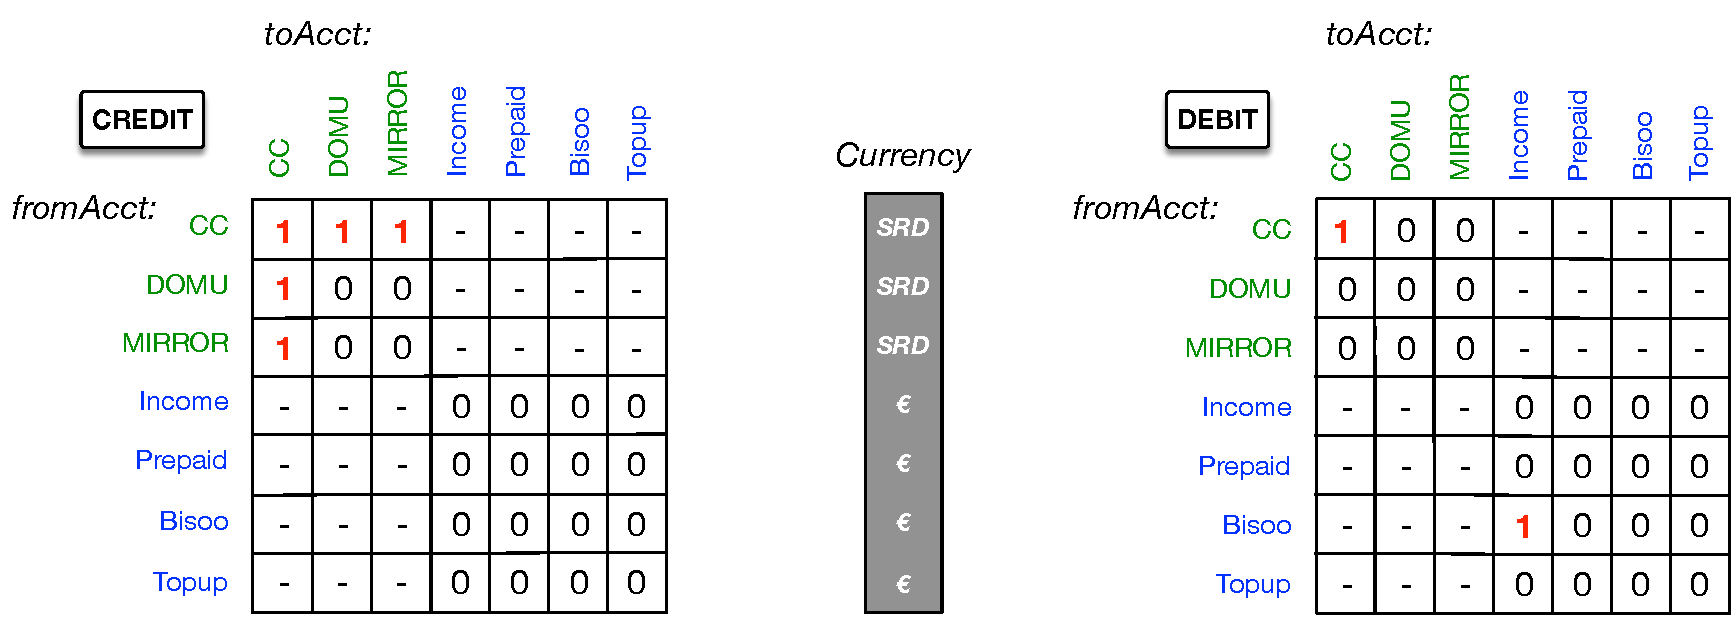
\includegraphics[width=16cm]{Figures/User_Acct_Connectivity}
\caption{\small\textbf{Account connectivity for user-initiated transactions: Test 2 in Figure \ref{fig:transactabilitywkflow}}}
\label{fig:User_Acct_Connectivity}
\end{figure}

\begin{figure}[H]
\vspace{-0.5cm}
\centering
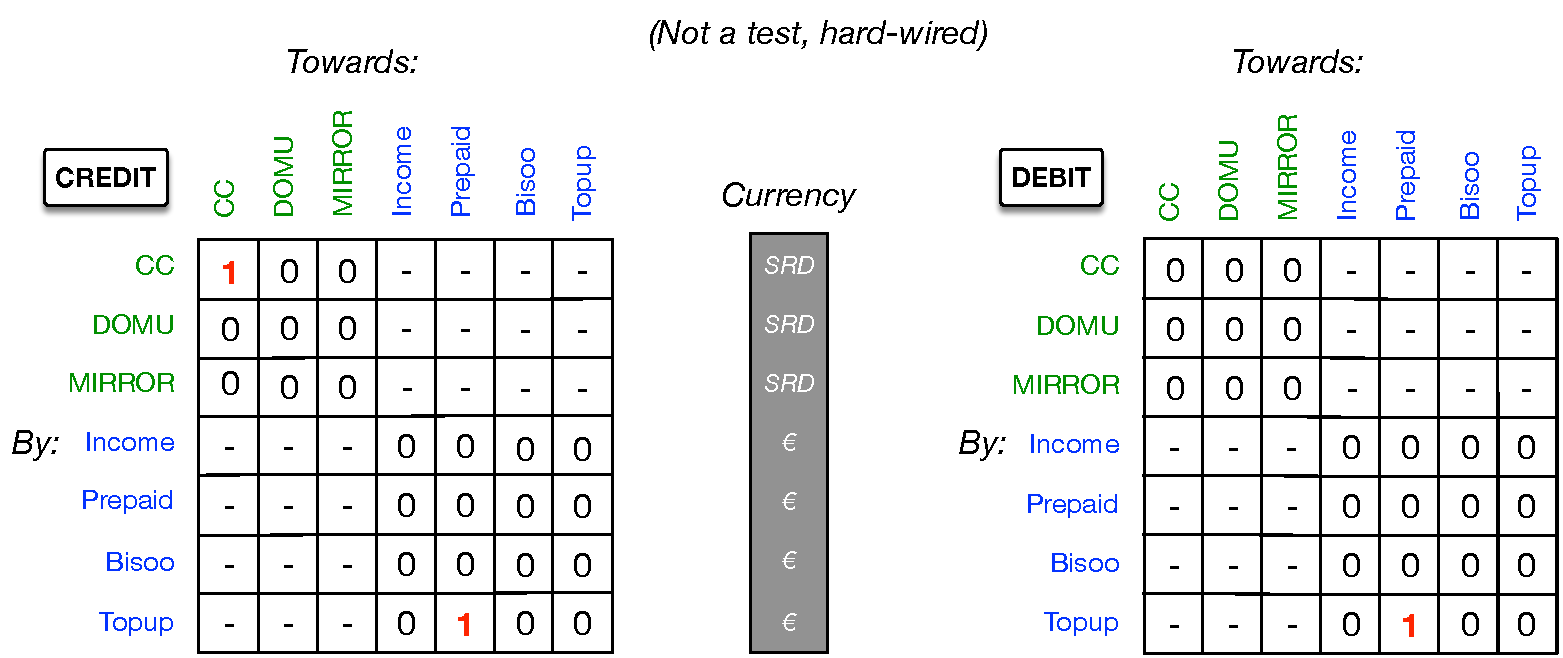
\includegraphics[width=16cm]{Figures/SysAdmin_Acct_Connectivity}
\caption{\small\textbf{Account connectivity for system-initiated transactions: Not a test, hard-wired. }}
\label{fig:SysAdmin_Acct_Connectivity}
\end{figure}

Figure \ref{fig:SysAdmin_Acct_Connectivity} shows a similar connectivity function for accounts that are controlled by $SysAdmin$. In this case, however, this function does not imply a transactability test since the permissions are hard-wired and SysAdmin does not need to test for transactability.

\subsection{User Transactability Functions}
\textbf{\small Note: this section has no bearing on the implementation, it is included to help interpret Figure \ref{fig:stack}.}

Figures \ref{fig:UTF1}-\ref{fig:UTF4} show a visualization of the interactions relevant to Layer 1 of Figure \ref{fig:stack}, filtered by the Account Connectivity constraints.

\begin{figure}[h]
\vspace{-0.5cm}
\centering
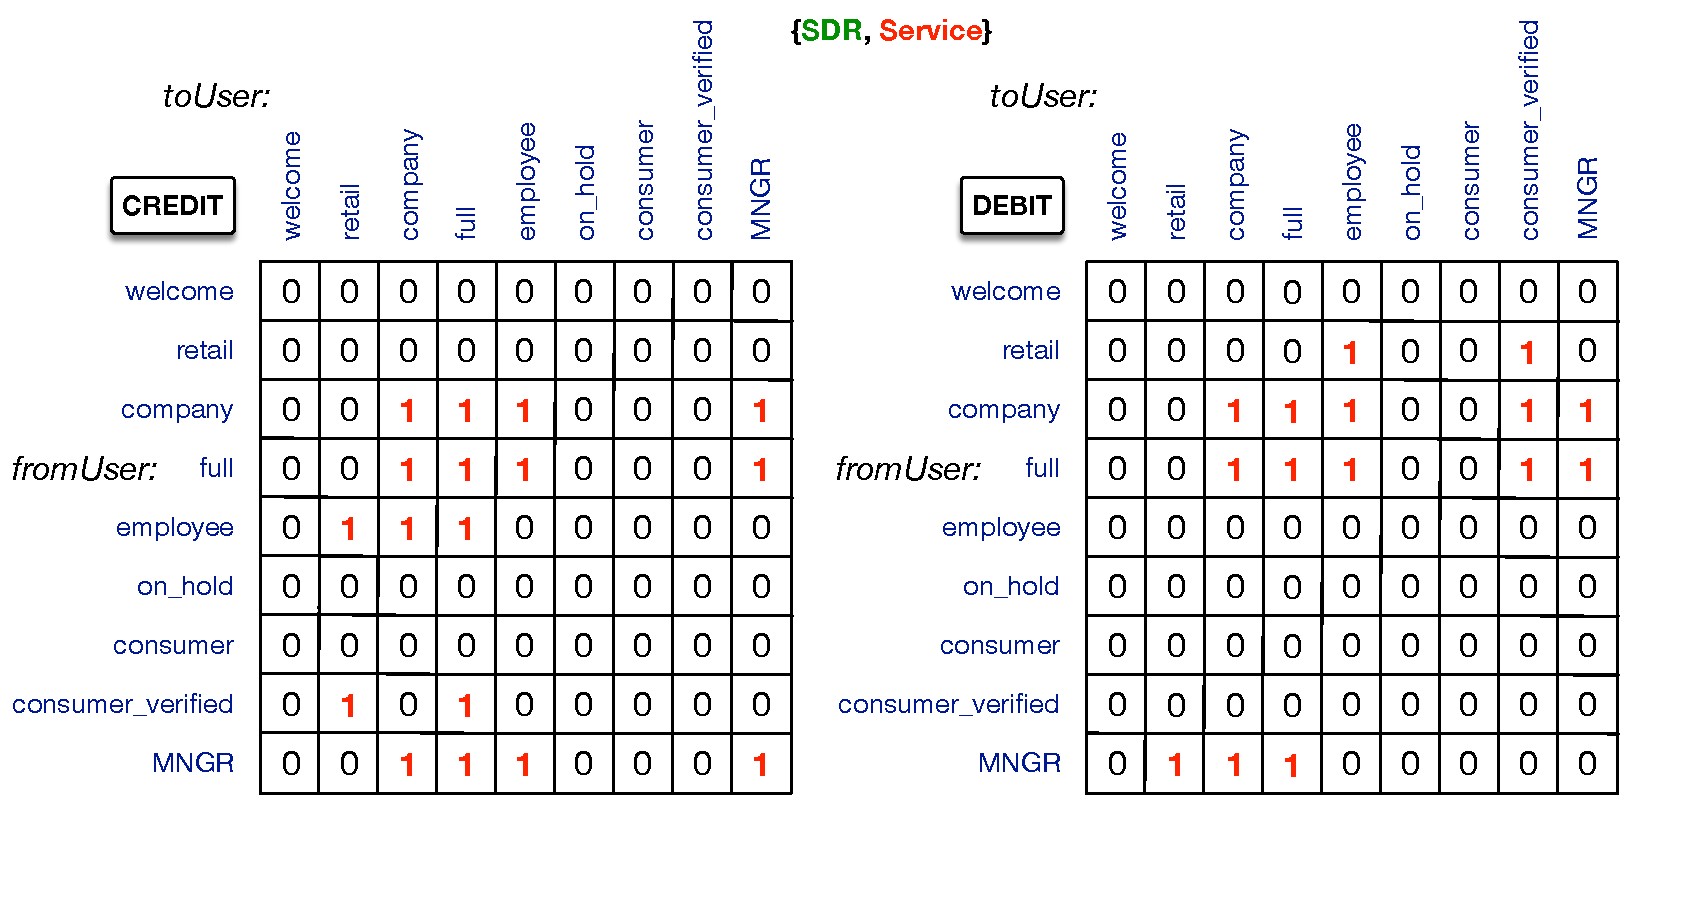
\includegraphics[width=17.5cm]{Figures/UTF1}
\caption{\small\textbf{User Transactability Function 1}}
\label{fig:UTF1}
\end{figure}

\begin{figure}[h]
\centering
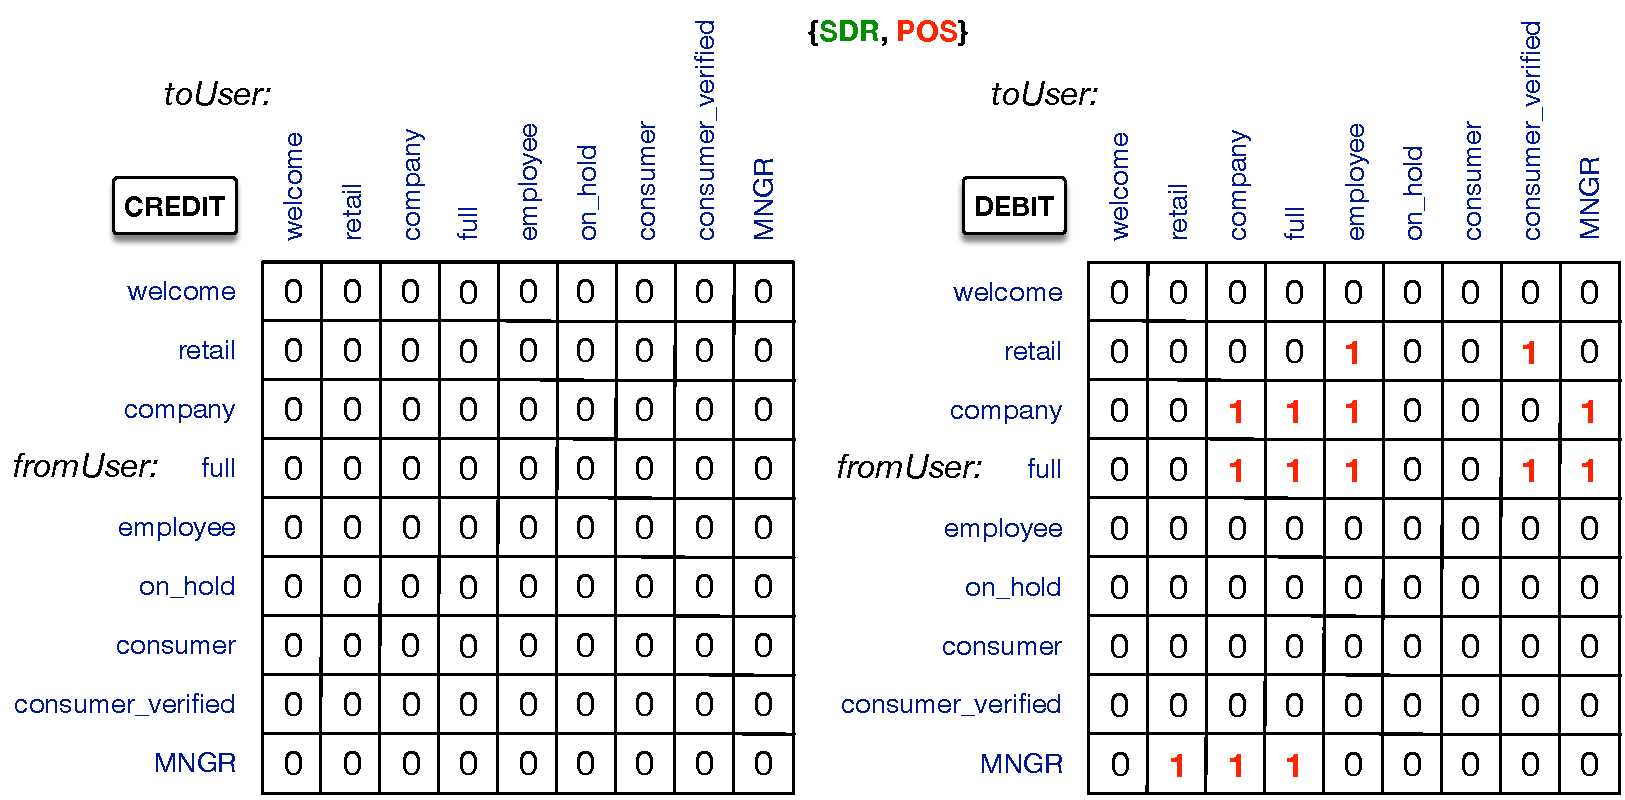
\includegraphics[width=17.5cm]{Figures/UTF2}
\caption{\small\textbf{User Transactability Function 2}}
\label{fig:UTF2}
\end{figure}

\begin{figure}[H]
\vspace{-0.5cm}
\centering
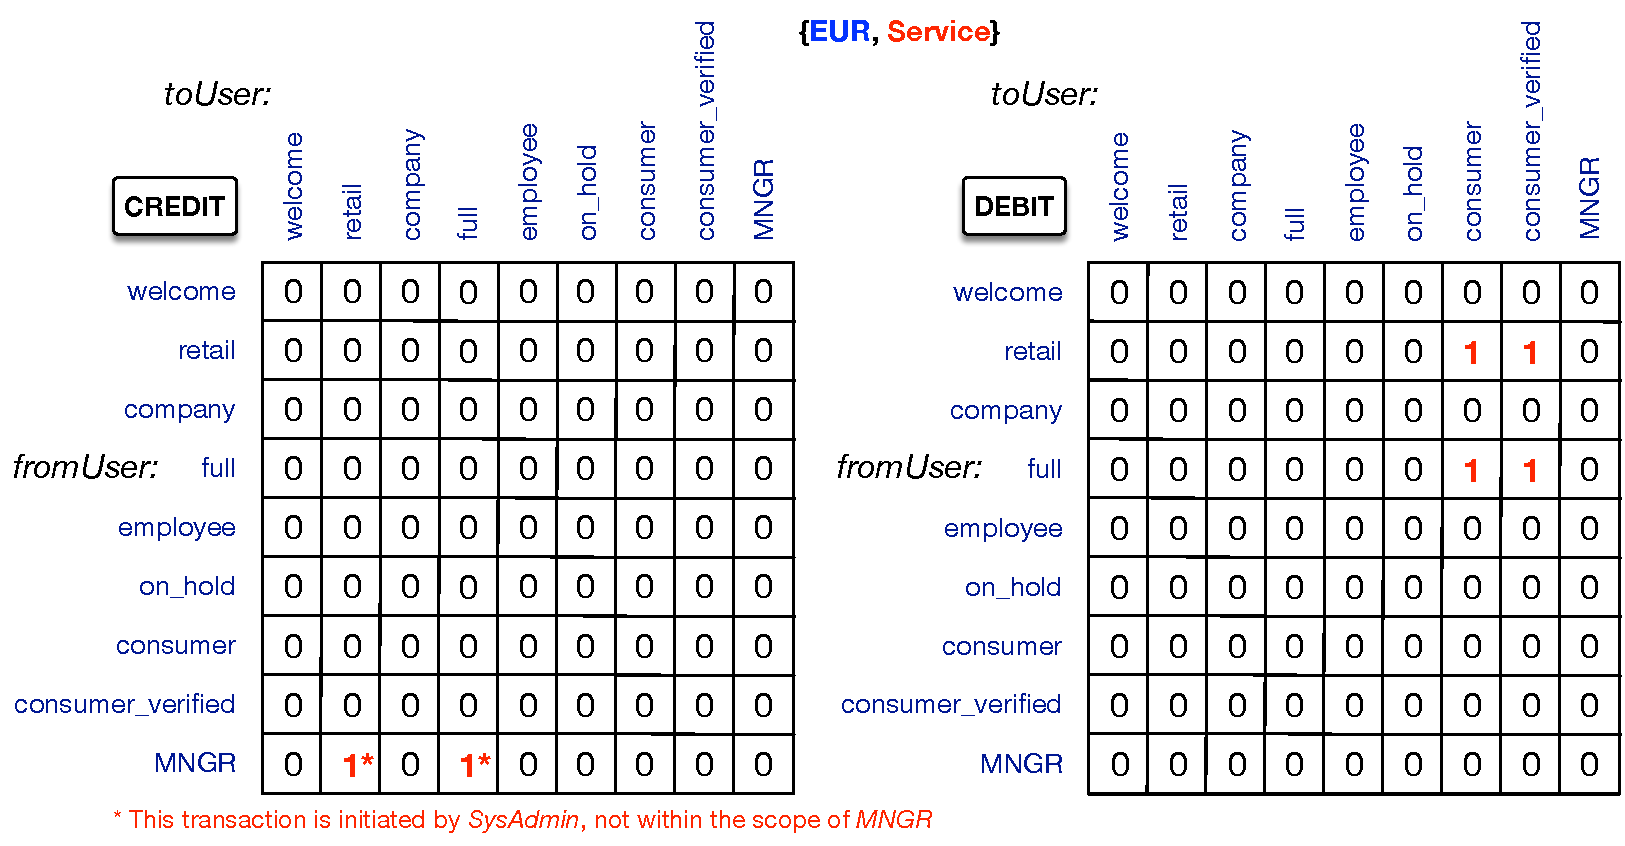
\includegraphics[width=17.5cm]{Figures/UTF3}
\caption{\small\textbf{User Transactability Function 3}}
\label{fig:UTF3}
%\vspace{-1cm}
\end{figure}

\begin{figure}[H]
\centering
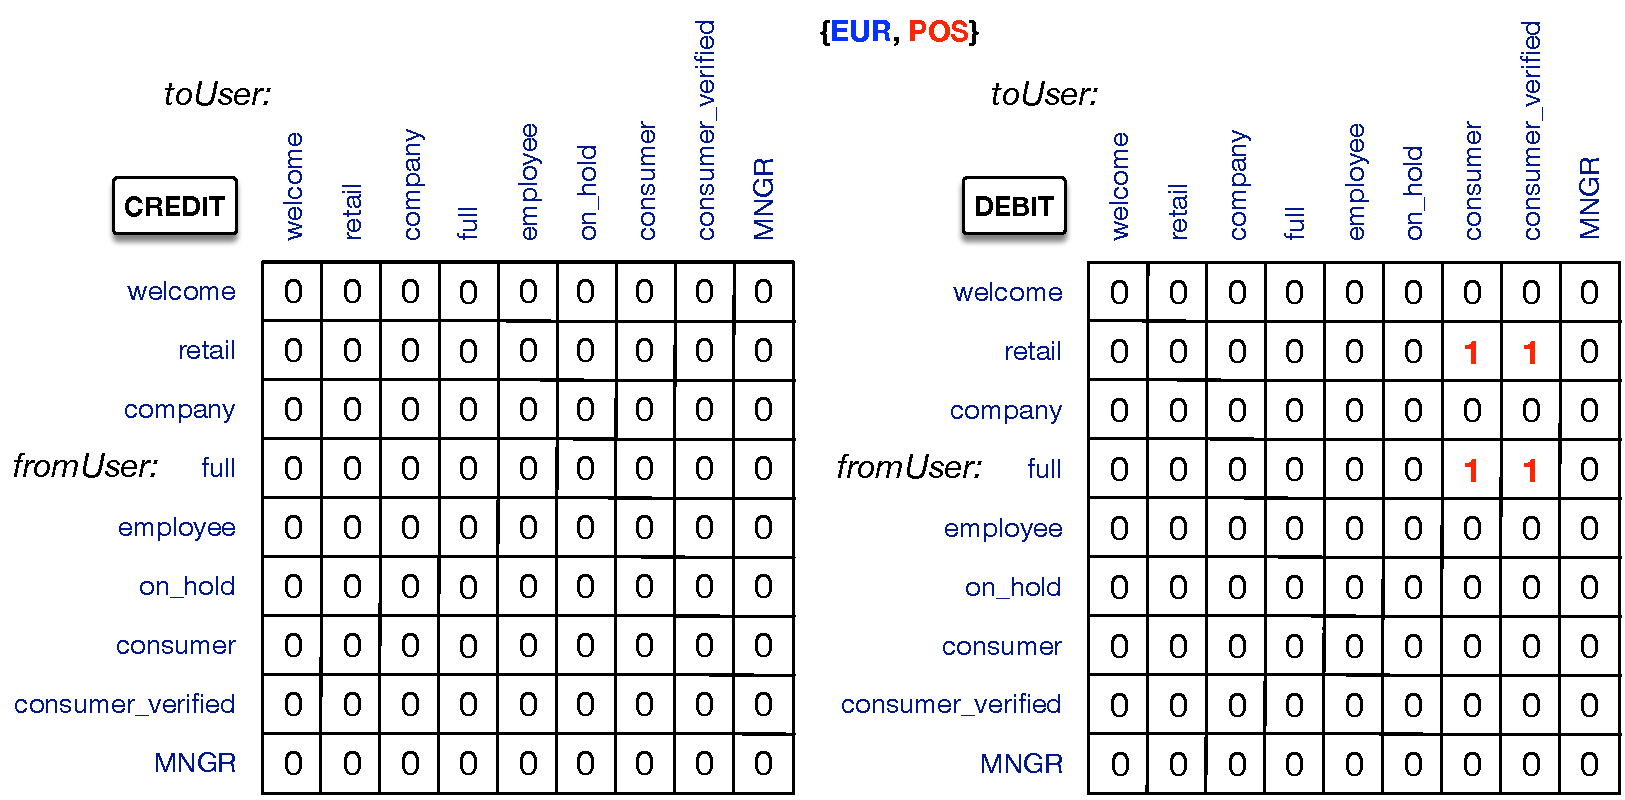
\includegraphics[width=17.5cm]{Figures/UTF4}
\caption{\small\textbf{User Transactability Function 4}}
\label{fig:UTF4}
\end{figure}



\subsection{Group Transactability Functions}
\textbf{\small Note: this section has no bearing on the implementation, it is included to help interpret Figure \ref{fig:stack}.}

The effect of the Transfer Types test together with the Account Connectivity test results in what we call the Group Transactability Function (GTF). Since there are 4 combinations of currency and channel, there are 4 different GTFs. There is no need to use them as an additional test, since they do not add anything new to Tests 1 and 2 of Figure \ref{fig:transactabilitywkflow}. However, it is still useful to include them here as another visualization of these first two tests of the Permissioning workflow, see Figures \ref{fig:GTF1}-\ref{fig:GTF4}.
\newpage

\vspace*{1cm}
\begin{figure}[h]
\centering
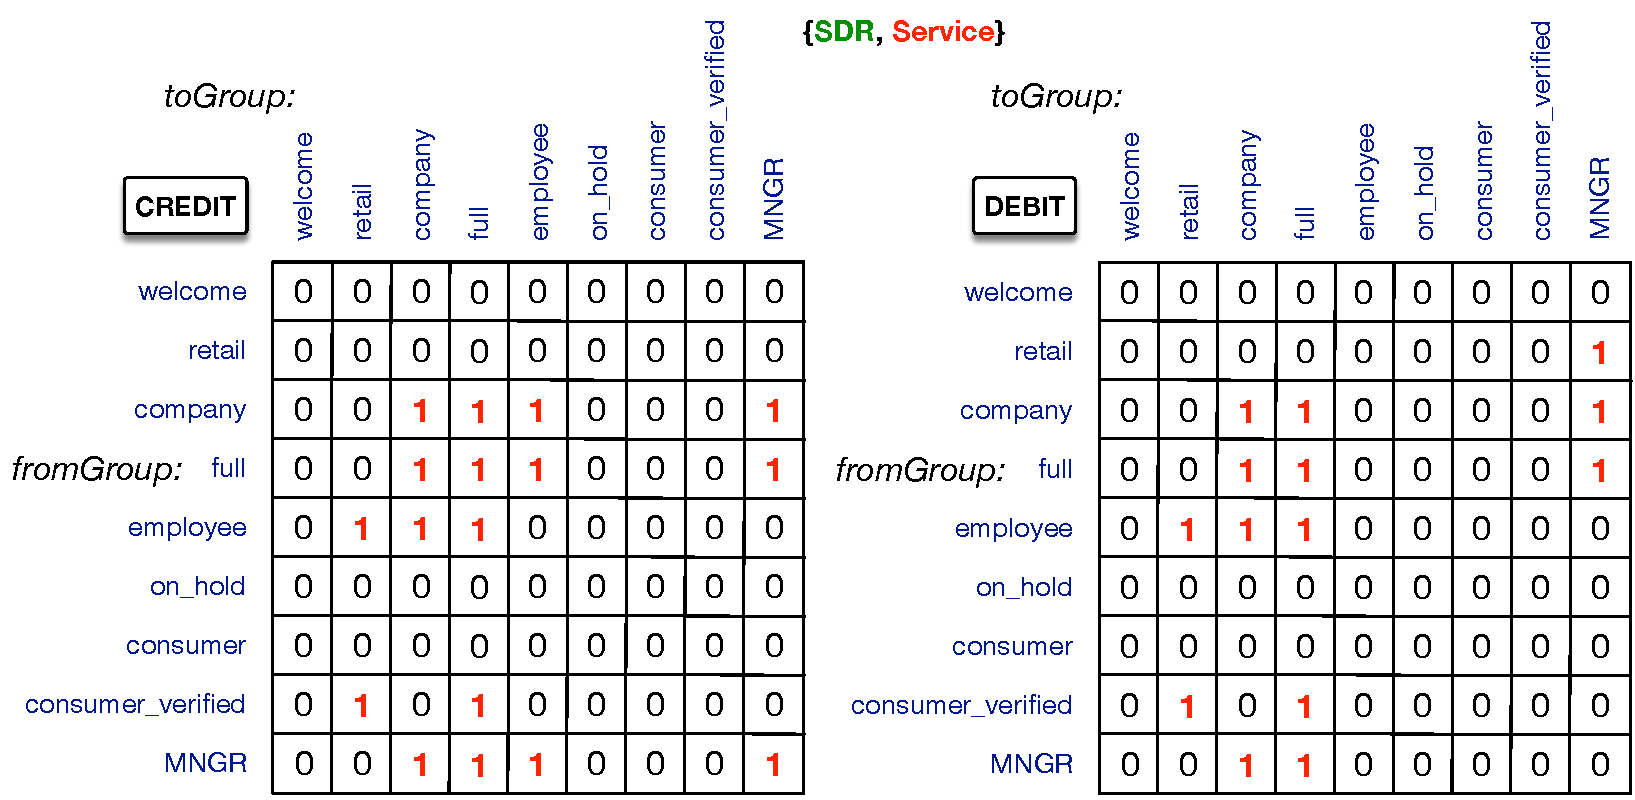
\includegraphics[width=17.5cm]{Figures/GTF1}
\caption{\small\textbf{Group Transactability Function 1}}
\label{fig:GTF1}
\end{figure}

\vspace*{2cm}

\begin{figure}[h]
\centering
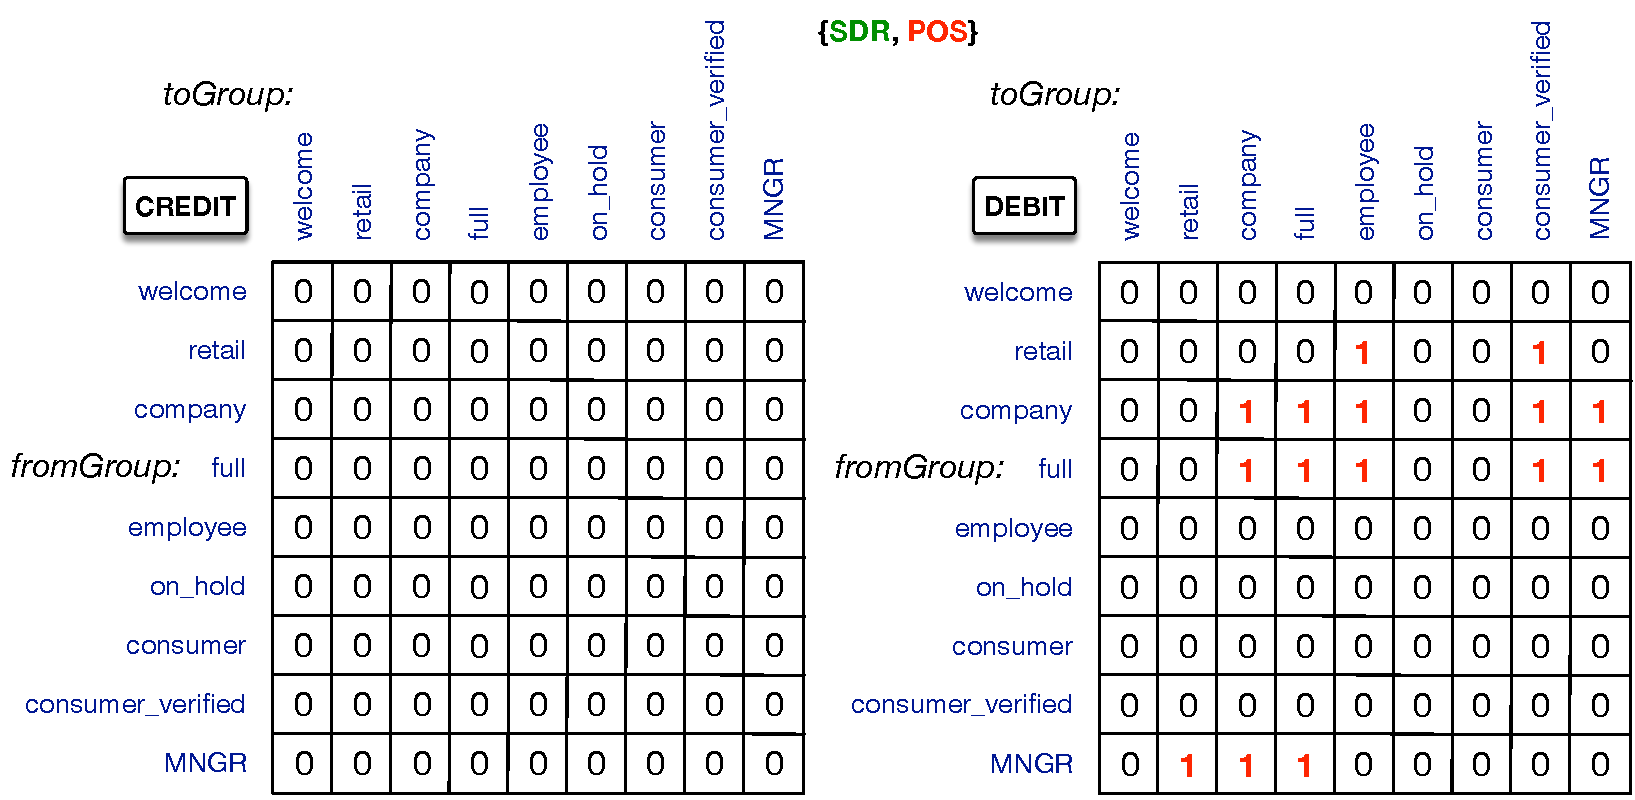
\includegraphics[width=17.5cm]{Figures/GTF2}
\caption{\small\textbf{Group Transactability Function 2}}
\label{fig:GTF2}
\end{figure}
%\vspace*{0.5cm}
\newpage

\begin{figure}[H]
%\vspace{-0.5cm}
\centering
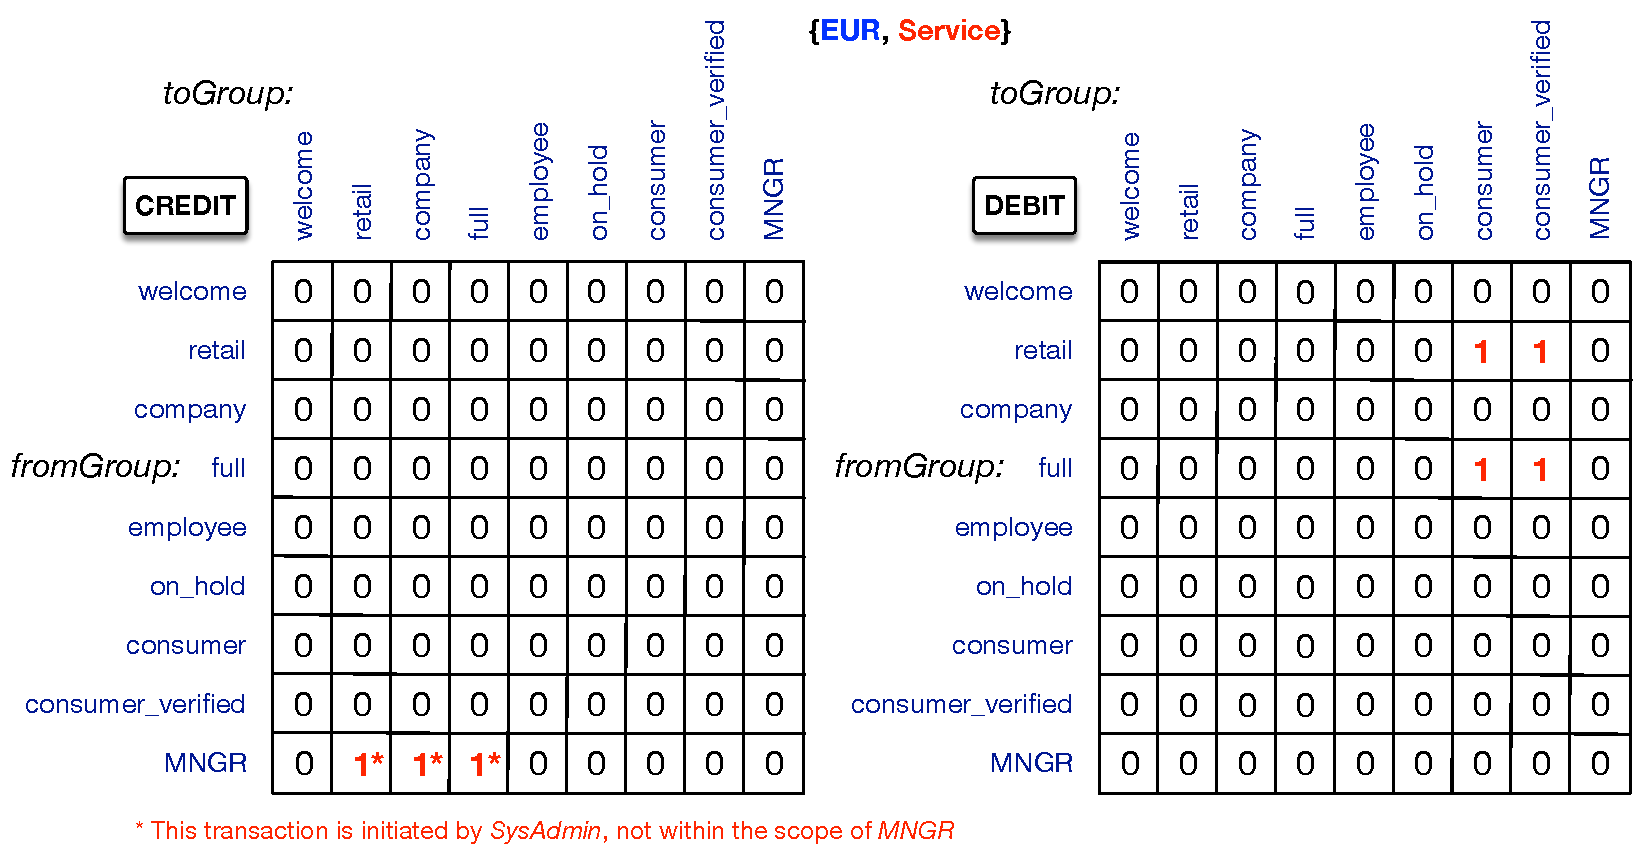
\includegraphics[width=17.5cm]{Figures/GTF3}
\caption{\small\textbf{Group Transactability Function 3}}
\label{fig:GTF3}
%\vspace{-1cm}
\end{figure}

\begin{figure}[H]
\centering
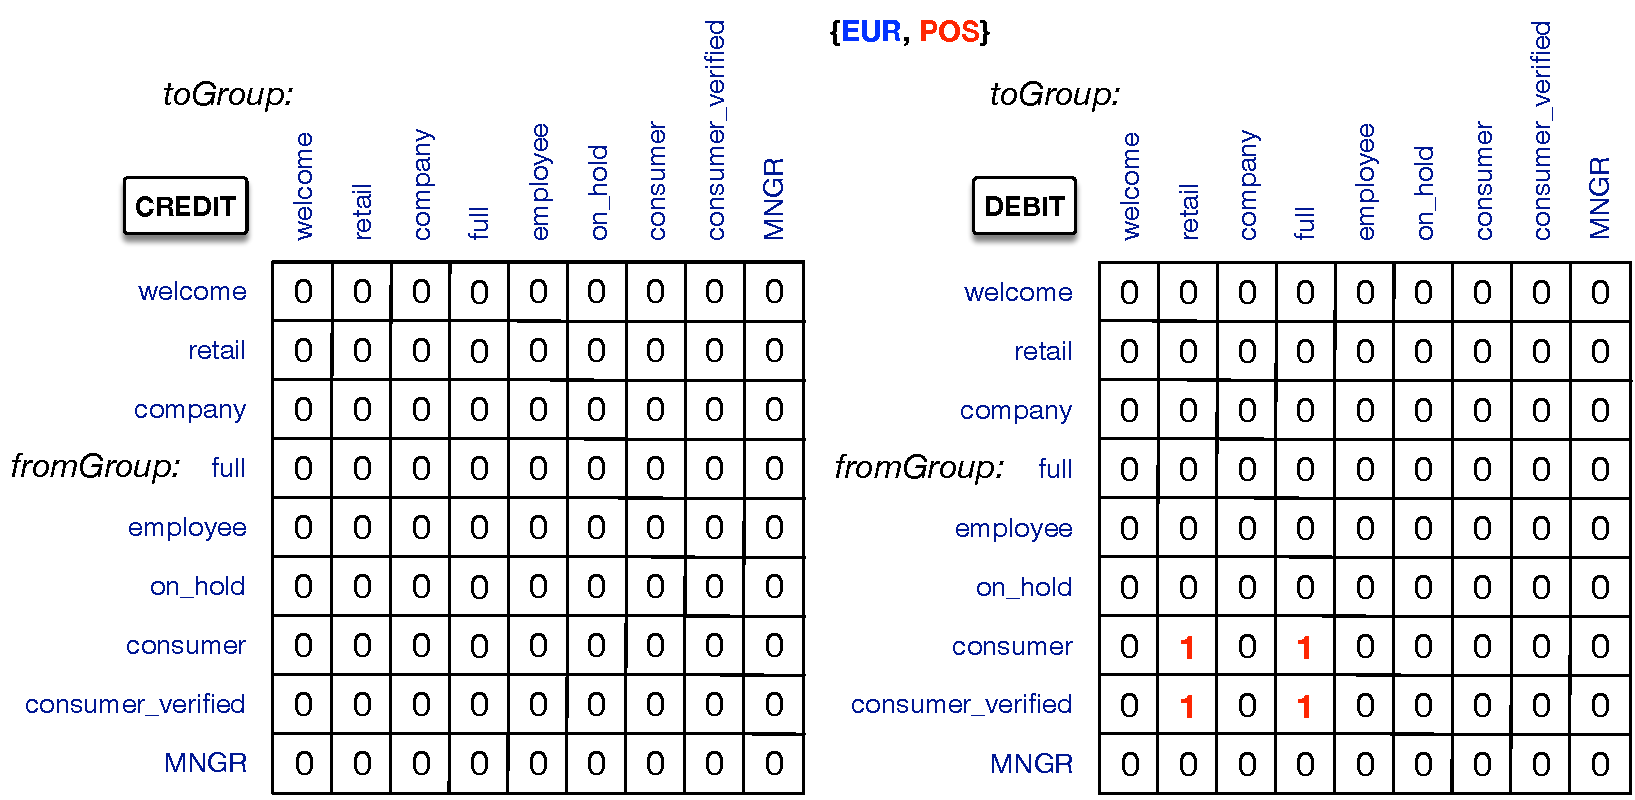
\includegraphics[width=17.5cm]{Figures/GTF4}
\caption{\small\textbf{Group Transactability Function 4}}
\label{fig:GTF4}
\end{figure}



\subsection{Transaction MetaData}

The transaction meta-data consists of only 1 memo message that is to be implemented as part of the transaction. It is not obligatory, i.e.\ the initiator of the transaction can leave it blank. The length is to be determined at the time of implementation but the assumption is that it is ``long enough'' to support a reasonable description of the transaction.

\newpage

\subsection{Account MetaData}
Tables \ref{tab:AccountMetaData1} and \ref{tab:AccountMetaData2} are also organized in terms of obligatory and optional meta-data, where the latter are modifiable by the user. At the implementation stage, for example, the modifiable fields can be included together with the profile meta-data. The fields that can be set by the user are indicated with an asterisk.

\begin{table}[H]
\begin{centering}
\small
{
\begin{tabular}{ r | c | l | l }
\hline
\textbf{Account}	& {\bf Account MetaData} & {\bf Type} & {\bf Description} \\
\Xhline{1.5pt}
			 & \emph{(Obligatory MetaData)}& & \\
\cline{2-2}
$CC$		& {\bf accountID}			&Integer	& Unique account identifier \\
			& {\bf memberID}			&String	& ProfileID of account owner \\
			& {\bf unit}					&String	& Account currency \\
			& {\bf balance}				&Double	& Account balance (positive or negative) \\
			& {\bf creditLimit}			&Double	& Credit limit (positive number) \\
			& {\bf creditLimitDate}		&DateTime & Date at which credit limit was set \\
			& {\bf availableBalance}		&Double	& $balance + creditLimit$ (non-negative number) \\
			& {\bf upperLimit}			&Double	& Upper balance limit (positive number) \\
			& {\bf availableCapacity}		&Double	& $capacity - saleVolume$ (non-negative number) \\
\cline{2-2}
			 & \emph{(Optional MetaData)}& & \\
\cline{2-2}
			& {\bf lowBalanceAlert$^*$}		&String	& Alert if $(creditLimit + balance) < lowBalanceAlert$ buffer \\
			& {\bf highBalanceAlert$^*$}		&String	& Alert if $(upperLimit - balance) < highBalanceAlert$ buffer \\
			& {\bf highVolumeAlert$^*$}		&String	& Alert if $(capacity - saleVolume) < highVolumeAlert$ buffer \\
\Xhline{1.5pt}
			 & \emph{(Obligatory MetaData)}& & \\
\cline{2-2}
$DOMU$		& {\bf accountID}			&Integer	& Unique account identifier \\
			& {\bf memberID}			&String	& ProfileID of account owner \\
			& {\bf unit}					&String	& Account currency \\
			& {\bf balance}				&Double	& Account balance (positive or negative) \\
			& {\bf creditLimit}			&Double	& Credit limit (positive number) \\
			& {\bf creditLimitDate}		&DateTime & Date at which credit limit was set \\
			& {\bf availableBalance}		&Double	& $balance + creditLimit$ (non-negative number) \\
\Xhline{1.5pt}
			 & \emph{(Obligatory MetaData)}& & \\
\cline{2-2}
$MIRROR$ 	& {\bf accountID}			&Integer	& Unique account identifier \\
			& {\bf memberID}			&String	& ProfileID of account owner \\
			& {\bf unit}					&String	& Account currency \\
			& {\bf balance}				&Double	& Account balance (positive or negative) \\
			& {\bf creditLimit}			&Double	& Credit limit (positive number) \\
			& {\bf creditLimitDate}		&DateTime & Date at which credit limit was set \\
			& {\bf availableBalance}		&Double	& $balance + creditLimit$ (non-negative number) \\
			& {\bf upperLimit}			&Double	& Upper balance limit (positive number) \\
			& {\bf availableCapacity}		&Double	& $capacity - saleVolume$ (non-negative number) \\
\cline{2-2}
			 & \emph{(Optional MetaData)}& & \\
\cline{2-2}
			& {\bf lowBalanceAlert$^*$}		&Double	& Alert if $(creditLimit + balance) < lowBalanceAlert$ buffer \\
			& {\bf highBalanceAlert$^*$}		&Double	& Alert if $(upperLimit - balance) < highBalanceAlert$ buffer \\
			& {\bf highVolumeAlert$^*$}		&String	& Alert if $(capacity - saleVolume) < highVolumeAlert$ buffer \\
\Xhline{1.5pt}
$Income$ 		& {\bf accountID}			&Integer	& Unique account identifier \\
			& {\bf memberID}			&String	& ProfileID of account owner \\
			& {\bf unit}					&String	& Account currency \\
			& {\bf balance}				&Double	& Account balance (positive or negative) \\
\Xhline{1.5pt}
\end{tabular}
}
\caption{\small\textbf{MetaData for $CC$, $DOMU$, $MIRROR$, and $Income$ accounts}\\
($^*$Indicates fields that can be modified by the user)}
\label{tab:AccountMetaData1}
\end{centering}
\end{table}

\begin{table}[H]
\begin{centering}
\small
{
\begin{tabular}{ r | c | l | l }
\hline
\textbf{Account}	& {\bf Account MetaData} & {\bf Type} & {\bf Description} \\
\Xhline{1.5pt}
			 & \emph{(Obligatory MetaData)}& & \\
\cline{2-2}
$Prepaid$ 	& {\bf accountID}			&Integer	& Unique account identifier \\
			& {\bf memberID}			&String	& ProfileID of account owner \\
			& {\bf unit}					&String	& Account currency \\
			& {\bf balance}				&Double	& Account balance (positive or zero) \\
			& {\bf creditLimit}			&Double	& Credit limit {\bf (Value can only be 0!)} \\
\cline{2-2}
			 & \emph{(Optional MetaData)}& & \\
\cline{2-2}
			& {\bf lowBalanceAlert$^*$}		&Double	& Alert if $(creditLimit + balance) < lowBalanceAlert$ buffer \\
\Xhline{1.5pt}
$Bisoo$ 		& {\bf accountID}			&Integer	& Unique account identifier \\
			& {\bf memberID}			&String	& ProfileID of account owner \\
			& {\bf unit}					&String	& Account currency \\
\Xhline{1.5pt}
$Topup$ 		& {\bf accountID}			&Integer	& Unique account identifier \\
			& {\bf memberID}			&String	& ProfileID of account owner \\
			& {\bf unit}					&String	& Account currency \\
\Xhline{1.5pt}
\end{tabular}
}
\caption{\small\textbf{MetaData for $Prepaid$, $Bisoo$, and $Topup$ accounts}\\
($^*$Indicates fields that can be modified by the user)}
\label{tab:AccountMetaData2}
\end{centering}
\end{table}

\section{Account Limit Tests}
The account limit tests are specified abstractly in D2.1. In the context the description of this chapter, which is closer to the implementation, they are fairly obvious by looking at Figures \ref{fig:accountLimitsCC} and \ref{fig:accountLimitsPrepaid}. The important thing is that they need to be enforced \emph{before} a transaction is completed. If one of the tests fails the transaction is not executed and the user must be alerted.

The alerts, on the other hand, can be issued \emph{after} a transaction that came close to a limit but did not cross it, if the resulting balance or sale volume exceeds the buffer limits.



























